\documentclass[a4paper, twoside, 12pt, czech]{article}
\usepackage[czech]{babel}
\usepackage{latexsym}
\usepackage{titlesec}
%\usepackage{ulem}
\usepackage{graphicx}
\usepackage{csquotes}
\usepackage[table,xcdraw]{xcolor}
\usepackage{tikz, pgfplots, mathtools}
\usepackage{microtype}
\usepackage[
    backend=biber,
    citestyle=nejm,
    bibstyle=iso-authoryear,
    sorting=none,
    spacecolon=false,
    labeldateparts=true,
    ]{biblatex}
\defbibenvironment{bibliography}
  {\list
     {\printtext[labelnumberwidth]{%
        \printfield{labelprefix}%
        \printfield{labelnumber}}}
     {\setlength{\labelwidth}{\labelnumberwidth}%
      \setlength{\leftmargin}{\labelwidth}%
      \setlength{\labelsep}{\biblabelsep}%
      \addtolength{\leftmargin}{\labelsep}%
      \setlength{\itemsep}{\bibitemsep}%
      \setlength{\parsep}{\bibparsep}}%
      \renewcommand*{\makelabel}[1]{\hss##1}}
  {\endlist}
  {\item}

% 1. Odstraní závorky kolem roku v seznamu literatury
\DeclareFieldFormat{biblabeldate}{#1}

% 2. Nastaví tečku a mezeru MEZI autorem a rokem (místo výchozí mezery)
\DeclareDelimFormat[bib]{nameyeardelim}{\addperiod\space}

% 3. Pro jistotu nastaví tečku a mezeru ZA rokem (před názvem díla)
\DeclareDelimFormat[bib]{nametitledelim}{\addperiod\space}

% 1. Čárka mezi více autory (nahradí středník/pomlčku)
\DeclareDelimFormat[bib]{multinamedelim}{\addcomma\space}

% 2. Spojka "a" před posledním autorem (pokud tam chceš taky čárku, přepiš to na \addcomma\space)
\DeclareDelimFormat[bib]{finalnamedelim}{\addcomma\space}

\DefineBibliographyStrings{czech}{
  urlalso = {Dostupné z\addcolon},
  urlfrom = {Dostupné z\addcolon}
}


%\DeclareNameAlias{sortname}{family-given}
\addbibresource{citace.bib}
\definecolor{myblue}{RGB}{52, 152, 219}
\usepackage{times}
\usepackage{coffeestains}
\usepackage{indentfirst}
\usepackage{fancyvrb}
\usepackage{keyboard}

\usepackage{newfloat}
\usepackage{float}
\usepackage[acronym]{glossaries} % Načtení balíčku s podporou akronymů
\usetikzlibrary{arrows.meta, positioning, shapes.geometric, automata}

\renewcommand{\thefootnote}{\roman{footnote}}

% Definice nového typu objektu "graph"
\DeclareFloatingEnvironment[
    fileext=logr,   % přípona pomocného souboru (libovolná, např. list of graphs)
    listname={Seznam grafů},
    name={Graf},
    placement=tp,   % preferované umístění (top, page)
]{graph}

% Pokud používáš češtinu přes babel, můžeš názvy doladit takto:
\addto\captionsczech{
  \renewcommand{\graphname}{Graf}
  \renewcommand{\listgraphname}{Seznam grafů}
}

\usepackage[hidelinks]{hyperref}
\usepackage{pdfpages}

\author{František SCHENK}
\title{Optimalizace rozložení kláves na klávesnici pro psaní v českém jazyce}
\date{2026}
\frenchspacing
\linespread{1.25}

\titleformat{\chapter}[display]{\normalfont\bfseries}{}{0pt}{\Huge\thechapter.\ } % Tenhle příkaz maže obrovský nápis KAPITOLA před každou kapitolou
\renewcommand{\floatpagefraction}{.8}%

\makeatletter
\newcommand \Dotfill {\leavevmode \cleaders \hb@xt@ .75em{\hss .\hss }\hfill \kern \z@}
\makeatother
% Konec preambule

\begin{document}
\begin{titlepage}
    \begin{center}
        \Huge
        \textbf{Česká zemědělská univerzita v~Praze}
        
        \vspace{0.5cm}
        \textbf{Provozně ekonomická fakulta}

        \vspace{0.5cm}
        \LARGE\textbf{Katedra informačního inženýrství}

        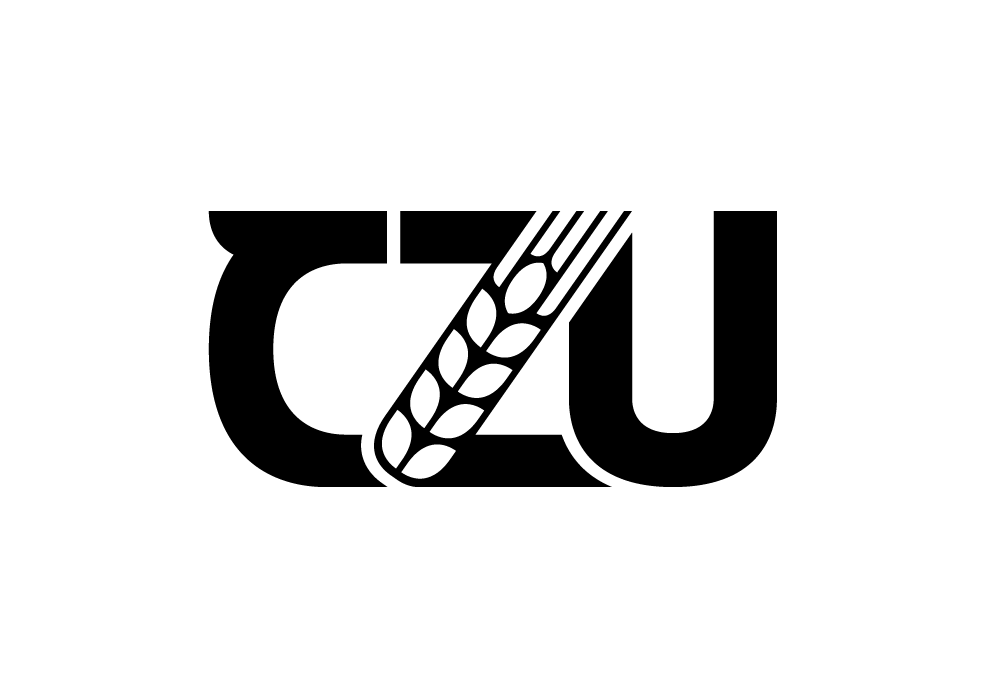
\includegraphics[width=0.8\textwidth]{obrazky/czuLogo.png}


        \vspace{0.5cm}
        \textbf{Diplomová práce}

        \vspace{0.5cm}
        \Large{Optimalizace rozložení kláves na klávesnici pro psaní v~českém jazyce}
        
        \vspace{0.5cm}
        \textbf{František SCHENK}

        \vspace{2.1cm}
        \textbf{© 2026 ČZU v~Praze}

    \end{center}
\end{titlepage}
\includepdf[pages={1,2}]{zadani.pdf}
\newpage

\newpage
\thispagestyle{empty}
\mbox{}
\vfill
\textbf{Čestné prohlášení}
\vspace{0.5cm}

Prohlašuji, že svou diplomovou práci ''Optimalizace rozložení kláves na kláves\-nici pro psaní v českém jazyce'' jsem vypracoval samostatně pod vedením vedoucího diplomové práce a~s použitím odborné literatury a~dalších informačních zdrojů, které jsou citovány v~práci a~uvedeny v~seznamu použitých zdrojů na konci práce. Jako autor uvedené diplomové práce dále prohlašuji, že jsem v~souvislosti s~jejím vytvořením neporušil autorská práva třetích osob.

\vspace{1.5cm}
V Praze dne 23.3.2026
\hspace{4cm}
\begin{tikzpicture}
    \draw(0,0) -- (4,0);
\end{tikzpicture}

\newpage
\thispagestyle{empty}
\mbox{}
\vfill
\textbf{Poděkování}
\vspace{0.5cm}

Tímto děkuji svému vedoucímu Ing. Davidovi Buchtelovi, Ph.D. za vedení práce, 
a~Ivaně za podporu.

\newpage
\noindent\Large\textbf{Optimalizace rozložení kláves na klávesnici pro psaní v českém jazyce}

\vspace{1cm}
\normalsize
\noindent\textbf{Abstrakt}

Diplomová práce se zabývá návrhem a optimalizací nového rozložení kláves\-nice 
specificky pro český jazyk s využitím metaheuristických algoritmů. Cílem je 
minimalizace biomechanické náročnosti psaní a zvýšení ergonomického komfortu 
uživatele. Na základě analýzy korpusu české Wikipedie byly získány statistiky 
n-gramů, které sloužily jako vstup pro nákladovou funkci. V rámci práce bylo 
implementováno a porovnáno pět optimalizačních algoritmů, z nichž nejlepších 
výsledků dosáhl genetický algoritmus. Vítězné rozložení bylo následně validováno 
na fyzickém hardwarovém prototypu.

\vspace{0.5cm}
\noindent\textbf{Klíčová slova}: 

Ergonomie klávesnice, Český jazyk, Optimalizace rozložení klávesnice, N-gramová 
analýza, Problém uspořádání klávesnice (KAP), Metaheuristické algoritmy 

\newpage
\noindent\Large\textbf{Optimization of Keyboard Layout for Writing in Czech}

\vspace{1cm}
\normalsize
\noindent\textbf{Abstract}

The diploma thesis deals with the design and optimization of a new keyboard 
layout specifically for the Czech language using metaheuristic algorithms. 
The aim is to minimize the biomechanical demand of typing and increase the 
ergonomic comfort of the user. Based on the analysis of the Czech Wikipedia 
corpus, n-gram statistics were obtained, which served as input for the cost 
function. Within the framework of the thesis, five optimization algorithms were 
implemented and compared, among which the genetic algorithm achieved the best 
results. The winning layout was subsequently validated on a physical hardware 
prototype.

\vspace{0.5cm}
\noindent\textbf{Keywords}: 

Keyboard ergonomics, Czech language, Keyboard layout optimization, N-gram analysis,
Keyboard Arrangement Problem (KAP), Metaheuristic algorithms
\newpage
\tableofcontents
\newpage

\section{Úvod}
Ačkoli v posledních desetiletích dochází k neustálému a rychlému vývoji technologií 
v oblasti interakce mezi člověkem a počítačem, jako je rozpoznávání hlasu, rukopisu 
či využití dotykových obrazovek, abecední klávesnice zůstává i~nadále jedním 
z~nejrozšířenějších a~nejefektivnějších nástrojů pro zadávání velkého objemu textu
(\cite{applicationAlgo}, s. 2; \cite{textEntrySystems}, s. 189). 
Její každodenní používání je nezbytnou součástí pracovního i osobního života pro 
obrovské množství uživatelů (\cite{engramapproach}, s. 1). 
S narůstající dobou strávenou u počítačů se však do 
popředí dostává otázka ergonomie a s ní spojená zdravotní rizika. Opakované 
a~nepřirozené pohyby prstů a rukou při psaní na nevhodně navrženém rozhraní mohou 
vést k únavě, svalovému napětí a vzniku muskuloskeletálních poruch (MSD), jako 
je například syndrom karpálního tunelu (\cite{engramapproach}, s. 1; \cite{applicationAlgo}, s. 1).

Současným celosvětovým standardem je rozložení klávesnice QWERTY, 
respektive jeho národní modifikace, jakou je v českém prostředí QWERTZ (\cite{applicationAlgo}, s.~2; \cite{lockin}, s. 10). Počátky 
tohoto uspořádání sahají až do 70. let 19. století. Z historického kontextu i 
odborných analýz jasně vyplývá, že hlavním záměrem při vývoji QWER\-TY nebylo 
maximalizovat rychlost psaní nebo vytvořit ergonomicky ideální pros\-tředí pro 
uživatele, nýbrž překonat tehdejší mechanická omezení psacích strojů
(\cite{textEntrySystems}, s.~8-9). 
%Cílem bylo umístit písmena, která se v angličtině často vyskytují v párech (digramech), na opačné strany takzvaného typového koše, aby se při rychlém sledu úhozů předešlo srážce a zaseknutí mechanických pák.

Ačkoliv s nástupem elektronických psacích strojů a moderních počítačových či virtuálních 
klávesnic tento mechanický problém zcela vymizel, standard QWER\-TY (a z něj odvozené 
QWERTZ) přetrvává (\cite{qwerty-dilemma}, s. 1235). Tento jev je často označo\-ván jako závislost na cestě (path dependence) 
a uzamčení (lock-in), kdy tržní dominance a historická setrvačnost brání přechodu 
na objektivně efektivnější řešení. Z ergonomického hlediska je tradiční rozvržení 
značně nedokonalé (\cite{qwerty-dilemma}, s. 1233). Výzkumy ukazují, že při jeho používání dochází k nevyváženému 
zatížení rukou (levá ruka vykonává více práce než pravá), nadměrným přesunům prstů 
mezi řadami a naopak k nedostatečnému využití nejdostupnější, střední (domovské) řady 
kláves (\cite{qwerty-dilemma}, s. 1233; \cite{qwerty-immortal}, s. 118).

Snahy o vylepšení tohoto stavu vedly k vývoji ergonomičtějších alternativ, z~nichž 
nejznámější je Dvorakova zjednodušená klávesnice představená v roce 1936 (\cite{applicationAlgo}, s. 1), nebo novější 
uspořádání jako Colemak z roku 2006 (\cite{qwerty-dilemma}, s. 1235). Tyto klávesnice prokazatelně zkracují celkovou 
vzdálenost, kterou prsty při psaní urazí, čímž snižují námahu a zvyšují plynulost (\cite{qwerty-dilemma}, s. 1233; \cite{applicationAlgo}, s. 3). 
Zásadním problémem však je, že drtivá většina těchto vylepšených rozložení byla 
navržena a~optimalizována primárně pro anglický jazyk, a to za pomoci statistik 
anglických textových korpusů (\cite{applicationAlgo}, s. 1).

Uspořádání, které je vysoce efektivní pro jeden jazyk, ovšem zpravidla ztrácí na 
účinnosti v jazycích jiných. Frekvence výskytu jednotlivých písmen a zejména n-gramů 
(dvojic či trojic písmen bezprostředně po sobě jdoucích) se napříč světo\-vými jazyky 
významně liší (\cite{lockin}, s. 11; \cite{textEntrySystems}, s. 198). Statistická analýza n-gramů je přitom stěžejním prvkem pro návrh 
optimalizovaného uspořádání kláves, neboť právě častost po sobě jdoucích úhozů 
definuje, které klávesy by měly ležet v~těsné blízkosti, nebo ideálně umožňovat 
střídání levé a pravé ruky pro plynulejší kadenci (\cite{applicationAlgo}, s. 1; \cite{diagramBasedLayout}, s. 416). Aby bylo možné dosáhnout maximálního 
komfortu a minimalizovat zdravotní zátěž při psaní českých textů, je nezbytné navrhnout 
rozložení znaků reflektující specifické statistické charakteristiky českého jazyka.

Samotné hledání ideálního rozložení na předem definované mřížce znaků je v~literatuře 
definováno jako „problém uspořádání klávesnice“ (keyboard arrangement problem – KAP) (\cite{applicationAlgo}, s. 2). 
Jde o~kombinatorickou optimalizační úlohu, která se řadí do třídy NP-těžkých problémů (\cite{engramapproach}, s. 2). 
Pouze pro anglickou abecedu o~26 písmenech existuje více než 400 kvadriliard $(4\times10^{26})$
možných permutací rozložení, což činí nalezení absolutního optima analytickými metodami 
či metodou hrubé síly (brute force) v~reálném čase zcela neproveditelným (\cite{engramapproach}, s. 2). K~řešení 
tohoto obrovského stavového prostoru se proto využívají moderní metaheuristické 
algoritmy. Dosavadní studie ve světě s úspěchem aplikovaly techniky umělé inteligence, 
jako jsou genetické algoritmy (GA) (\cite{applicationAlgo}, s. 1), simulované žíhání 
(simulated annealing) (\cite{applicationAlgo}, s. 2) či 
algoritmy optimalizace mravenčí kolonií (ACO) (\cite{engramapproach}, s. 1).

Tato diplomová práce reaguje na absenci dedikovaného, na datech postaveného řešení 
pro české prostředí. Cílem práce je vytvořit a aplikovat metodiku pro návrh nového, 
ergonomicky optimalizovaného rozložení klávesnice pro psaní všemi deseti prsty, 
které je specificky přizpůsobeno českému jazyku. Dosažení tohoto cíle je podmíněno 
stanovením adekvátní nákladové (účelové) funkce, která kvantifikuje biomechanickou 
náročnost psaní zohledněním pohybů prstů na klávesnici, a~zpracováním rozsáhlého 
korpusu českých textů pro získání potřebných n-gramo\-vých statistik. Pro nalezení 
finálního řešení v komplexním prostoru možností je využito metaheuristických 
optimalizačních algoritmů. Výsledkem je návrh rozlo\-žení, jež má potenciál podstatně 
snížit dráhu pohybu prstů, redukovat fyzickou únavu uživatele a zefektivnit celkovou 
produkci textu v českém jazyce.
\newpage

\section{Cíl práce a metodika}
\subsection{Cíl práce}
Cílem diplomové práce je navrhnout a algoritmicky optimalizovat nové rozlo\-žení 
klávesnice pro efektivní a ergonomické psaní v českém jazyce, a to na základě 
frekvenční analýzy lingvistických dat a aplikace heuristických algoritmů. 
Existují sice alternativy ke klasickému QWERTY (nebo k lokalizovanému QWERTZ), například Dvorak, 
Colemak nebo Workman, ale ty nejsou vhodné pro jazyky s~větším množstvím 
diakritických znaků. Přestože alternativy nemusí zvýšit rychlost, mohou zvýšit 
pohodlí při psaní. Výstupem práce bude optimalizované rozlo\-žení klávesnice pro psaní 
v českém jazyce a sada algoritmů, které byly využity k~dosažení tohoto rozložení.

Pro dosažení hlavního cíle byly stanoveny následující dílčí kroky:
\begin{itemize}
    \item Provést frekvenční analýzu n-gramů na rozsáhlém korpusu českých textů.
    \item Definovat matematickou nákladovou funkci, která objektivně zohlední 
    anatomickou náročnost úhozů a plynulost psaní.
    \item Aplikovat a srovnat vybrané optimalizační algoritmy za účelem nalezení 
    optimálního rozložení.
    \item Zhodnotit a prakticky validovat nejlepší vygenerované rozložení na 
    hardwarovém prototypu klávesnice.
\end{itemize}
\subsection{Metodika}
%Budou aplikovány různé algoritmy na rozložení klávesnice, s cílem nalezení 
%alternativy ke QWERTZ. Mezi vhodné algoritmy patří algoritmy lokálního prohledávání 
%(například Hill Climbing nebo Simulated Annealing), genetické algoritmy, ACO a 
%PSO. Algoritmy budou implementovány v jazyce Python.

%Podle optimalizačních kritérií vznikne jedno nebo více rozložení s různými 
%výhodami a nevýhodami. Výsledky optimalizace budou během psaní práce 
%naprogramovány do klávesnice s QMK/Vial firmware. V závěru práce budou tato 
%rozložení zhodnocena z hlediska použitelnosti.

Pro potřeby sběru a zpracování lingvistických dat byl využit textový korpus české 
Wikipedie (\cite{wikidump}). Vzhledem k formátu, ve kterém je korpus dostupný, a jeho velikosti, 
byl korpus zpracován metodou inkrementálního parsování (anglicky stream processing).
Data byla následně očištěna o XML značky, písmena byla všechna převedena na malá,
a~došlo k odstranění dalších nadbytečných znaků. Výstupem pythonového skriptu pro 
zpracování dat byl seznam unigramů, digramů a trigramů s hodnotou jejich četnosti 
výskytu.

Následně byl stanoven hodnotící model, takzvaná nákladová funkce. Nejdříve byla 
navržena anatomická mapa klávesnice, která hodnotí každou klávesu na klá\-vesnici 
podle obtížnosti stisku kláves, a to tak, že jednodušeji dosažitelné řady a~sloupce 
dostaly nižší hodnocení než hůře dosažitelné klávesy. Nákladová funkce tedy 
musela být minimalizační, aby došlo k minimalizaci pohybu prstů napříč klávesnicí.
Nákladová funkce byla definována jako vážený součet unigramové a~trigramové zátěže,
s důrazem na plynulost sekvencí úhozů.

Pro hledání optimálního rozložení klávesnice byly v jazyce Python implementovány 
heuristické algoritmy. Mezi vybrané algoritmy patří horolezecký algoritmus, 
algoritmus simulovaného žíhání, optimalizace mravenčí kolonií, algoritmus optimalizace 
hejnem částic a genetický algoritmus. % s využitím metody křížení podle pořadí. 
Některá řešení bylo nutné rozšířit o~memetické varianty algoritmů, 
nebo kombinovat metody globálního prohledávání s algoritmy lokálního prohledávání 
pro dosažení přesnějších výsledků.

Za účelem praktického ověření použitelnosti bylo vítězné rozložení implementováno 
do mikrokontroleru testovací klávesnice s využitím open-source firmwaru QMK. Evaluace 
probíhala měřením rychlosti psaní a chybovosti v reálném čase, aby se prokázala 
(nebo vyvrátila) teoretická efektivita navrženého řešení.


%\coffeestainA{0.9}{0.85}{75}{5cm}{1.3cm}
\newpage
\section{Teoretická část práce}

Teoretická část práce shrnuje dosavadní poznatky nezbytné pro návrh 
optimalizovaného rozložení klávesnice. Úvodní kapitoly se věnují historickému 
kontextu vzniku standardu QWERTY a definují klíčové principy ergonomie práce s 
počítačem, které tvoří základ pro stanovení nákladové funkce. Následně je 
rozebrána struktura českého jazyka z pohledu n-gramů. Závěrečný úsek této 
části pak představuje vybrané optimalizační algoritmy, 
které jsou v praktické části využity pro hledání globálního optima.

\subsection{Vznik QWERTY}
Rozložení klávesnice QWERTY, které je dnes celosvětovým standardem pro vstup 
textu do počítačů a mobilních zařízení, má své kořeny v 60. a 70. letech 19. 
století. Jeho vznik je výsledkem složitého inženýrského procesu, který reagoval 
na mechanická omezení tehdejších psacích strojů a potřeby prvních uživatelů, kterými
byli telegrafisté.

Otcem psacího stroje a rozložení QWERTY je americký vynálezce Christopher Latham 
Sholes, který na vývoji spolupracoval s Carlosem Gliddenem, Samuelem W. Soulem 
a později s Jamesem Densmorem (\cite{prehistory}, s. 162). První prototypy, expedované v roce 1868, měly 
klávesnici připomínající klavír s 28 klávesami seřazenými abecedně (A–N, a obráceně O–Z) 
(\cite{prehistory}, s. 162), jak je vidět na obrázku \ref{pic:prvnikeeb}.
\begin{figure}[h]
    \centering
    % \textwidth = šířka textu na stránce
    % ! = výška se dopočítá automaticky, aby se zachoval poměr stran
    \caption{První prototyp telegrafické klávesnice}
    \vspace{0.5cm}
    \resizebox{\textwidth}{!}{%
        \begin{tikzpicture}[
            whitekey/.style={draw=black, fill=white, minimum width=1.2cm, minimum height=6cm, inner sep=0pt, outer sep=0pt, anchor=south west},
            blackkey/.style={draw=black, fill=black, minimum width=0.8cm, minimum height=3.5cm, inner sep=0pt, outer sep=0pt, anchor=north},
            whitelabel/.style={font=\sffamily\large, yshift=0.8cm},
            blacklabel/.style={font=\sffamily\large\bfseries, text=white, yshift=1.0cm}
        ]
            % ROZMĚRY (Tyto hodnoty teď slouží jen jako poměr, finální velikost určí resizebox)
            \def\wWidth{1.2}
            \def\wHeight{6}
            
            \def\WhiteKeys{ ,  , Z, Y, X, W, V, U, T, S, R, Q, P, O,  }
            \def\BlackKeys{A, B, C, D, E, F, G, H, I, J, K, L, M, N}

            % BÍLÉ
            \foreach \key [count=\i from 0] in \WhiteKeys {
                \node[whitekey] (w\i) at (\i*\wWidth, 0) {};
                \node[whitelabel] at (w\i.south east -| w\i.center) {\key};
            }

            % ČERNÉ
            \foreach \key [count=\i from 0] in \BlackKeys {
                \node[blackkey] (b\i) at ({(\i+1)*\wWidth}, \wHeight) {};
                \node[blacklabel] at (b\i.south) {\key};
            }
        \end{tikzpicture}%
    }
    
    \small{Zdroj: Vlastní zpracování podle (\cite{prehistory}, s. 162)}
    \label{pic:prvnikeeb}
\end{figure}

Koichi a spol. (\cite{prehistory}, s. 164) uvádí, že zásadní vliv na vývoj měli první zákazníci, kterými byli telegrafisté. 
Ti potřebovali stroj, který by dokázal rychle přepisovat přijímané Morseovy 
zprávy. V dubnu 1870 Sholes představil model s 38 klávesami ve čtyřech řadách, 
který se již blížil modernímu uspořádání, ačkoli byl stále do jisté míry abecední.
Zpětná vazba od telegrafistů vedla k dalším úpravám. Napří\-klad umístění písmena 
'S' blízko 'Z' a 'E' bylo pravděpodobně ovlivněno nejednoznačností americké 
Morseovy abecedy, kde kód pro 'Z' mohl být zaměněn za digram 'SE'. 
Telegrafisté proto potřebovali mít tato písmena blízko sebe pro rychlé rozlišení 
kontextu.

Rozšířeným mýtem je, že QWERTY bylo navrženo záměrně neefektivně, aby zpomalilo 
písaře a zabránilo tak zasekávání stroje. Historické analýzy a simulace však 
ukazují, že cílem nebylo zpomalit operátora, ale naopak umožnit plynulé psaní 
tím, že se předejde mechanickým kolizím (\cite{prehistory}, s. 161 ; \cite{qwerty-immortal}, s. 118).

V raných modelech (jako byl Remington No. 1) byly typové páky (typebars) 
zavěšeny v kruhovém koši a při stisku klávesy vyjížděly směrem nahoru do jednoho 
tiskového bodu (tzv. up-strike mechanismus) (\cite{lockin}, s. 5). Pokud byly stisknuty dvě sousední 
páky v rychlém sledu, mohly se srazit a zaseknout. Sholesovým řešením nebylo 
pouze oddělit časté dvojice písmen (digramy) na klávesnici, ale především 
zajistit, aby písmena, jejichž páky v mechanickém koši sousedí, tvořila v 
angličtině co nejméně frekventované dvojice. Tento koncept, nazývaný "princip 
nefrekventovanosti" (infrequency principle), umožnil umístit časté páry pák 
daleko od sebe, což minimalizovalo riziko zaseknutí (\cite{lockin}, s. 7; \cite{hidden-in-plain-sight}, s. 6).

Díky tomuto uspořádání bylo QWERTY z hlediska kompatibility formátu a~zařízení 
téměř optimálním řešením pro tehdejší technologii
(\cite{lockin}, s. 19). 
I kdyby bylo v té době k dispozici ergonomicky lepší rozlože\-ní (např. Dvorak), 
na mechanickém stroji s horním úderem by selhalo kvůli časté\-mu zasekávání
(\cite{qwertyoptimality}, s. 5).

V roce 1873 podepsali Sholes a Densmore smlouvu se zbrojovkou E. Remington \& 
Sons. Mechanici Remingtonu provedli finální úpravy, včetně přesunu písmene 'R' 
do horní řady (\cite{prehistory}, s. 165). Často se uvádí, že toto umožnilo prodejcům rychle napsat slovo 
"TYPE WRITER" pouze pomocí kláves v horní řadě, aby ohromili zákazníky, ačkoli 
někteří historici tuto teorii zpochybňují s tím, že název stroje existoval již 
dříve a ukázky probíhaly spíše formou diktátu (\cite{prehistory}, s. 172).

Klíčovým momentem pro ustálení QWERTY bylo uvedení modelu Remington No. 2 v roce 
1878, který jako první umožňoval psaní velkých i malých písmen pomocí klávesy 
Shift (\cite{qwerty-dilemma}, s. 1232; \cite{prehistory}, s. 161). V roce 1882 došlo k 
poslední drobné změně (přesun 'M' a prohození 'C' a 'X'), čímž vzniklo rozložení, 
které je využí\-váno dodnes (\cite{prehistory}, s. 168).

Dominanci QWERTY upevnilo zavedení hmatové metody psaní všemi deseti prsty 
(touch typing). Školy psaní na stroji začaly vyučovat psaní výhradně na strojích Remington s 
rozložením QWERTY (\cite{prehistory}, s. 168). V roce 1893 vytvořili hlavní výrobci psacích strojů 
(Remington, Caligraph, Yost, Densmore a Smith-Premier) trust Union Typewriter 
Company a přijali QWERTY jako standard. Do roku 1898 se QWERTY stalo 
univerzálním standardem (\cite{prehistory}, s. 169).

Při expanzi do Evropy bylo QWERTY upravováno podle stejného principu 
nefrekventovanosti, aby vyhovovalo specifickým frekvencím digramů v jiných 
jazycích. Tak vznikly varianty jako německé QWERTZ (kde je častější 'Z' a~vzácněj\-ší 'Y') 
nebo francouzské AZERTY a italské QZERTY (\cite{lockin}, s. 10). Analýzy ukazují, že 
tyto varianty byly pro své jazyky efektivnější než původní QWERTY (\cite{lockin}, s. 12).

Ačkoliv mechanické důvody pro QWERTY zmizely s příchodem psacích stro\-jů 
s~viditelným psaním (front-strike) kolem roku 1900 a později s nástupem 
elektrických strojů a počítačů, rozložení zůstalo nezměněno (\cite{lockin}, s. 19; 
\cite{hidden-in-plain-sight}, s. 2). Tento jev je v 
ekonomii nazýván závislostí na cestě (path dependence) a uzamčením (lock-in). 
Vysoké náklady na přeučení milionů písařů a výměnu hardwaru bránily přechodu na 
efektivnější systémy(\cite{lockin}, s. 4; \cite{hidden-in-plain-sight}, s. 2).

Nejznámějším vyzyvatelem byla Dvorakova zjednodušená klávesnice (DSK), 
patentovaná v roce 1936, která slibovala vyšší rychlost a menší únavu (\cite{applicationAlgo}, s. 1; 
\cite{qwerty-dilemma}, s.~1232). Přestože 
studie amerického námořnictva ze 40. let naznačovaly superioritu Dvoraka, 
pozdější analýzy (např. Liebowitz a Margolis) tyto výsledky zpochybnily a 
argumentovaly, že výhody nebyly dostatečné k tomu, aby ospravedlnily náklady na 
změnu (\cite{qwerty-dilemma}, s. 1233; \cite{lockin}, s. 19).

V moderní době QWERTY dominuje i na zařízeních, pro která nebylo navrže\-no, jako 
jsou dotykové obrazovky smartphonů, kde je psaní jedním prstem na tomto rozložení 
neefektivní (\cite{7814594}, s. 1). Přesto se QWERTY drží na pozici globální\-ho standardu 
díky síle zvyku a standardizaci. Tato dominantní pozice dokonce ovliv\-ňuje vnímání slov, jako například 
takzvaný „QWERTY 
efekt“, který ukazuje, že slova psaná více písmeny z pravé strany klávesnice jsou 
vnímána pozitivněji (\cite{qwerty-dilemma}, s.~1236).

\subsection{Ergonomie klávesnice}
%I přes nedávné pokroky v oblasti komunikace mezi člověkem a počítačem zůstává 
%klávesnice vysoko na žebříčku nejpoužívanějších vstupních zařízení. Nicméně 
%nadměrné nebo nesprávné  používání klávesnic může vést ke zranění z opakovaného 
%namáhání (anglicky repetitive strain injury - RSI).

%I. S. MacKenzie (\cite{textEntrySystems}) se tímto problémem zabýval a popsal 
%způsoby, jak těmto zraněním předcházet. Vyzdvihuje několik hlavních metod, 
%kterými lze předejít nadměrné únavě při psaní na klávesnici. Velkou roli hraje 
%poloha klávesnice, tedy výška stolu a úhel náklonu klávesnice jsou faktory, které 
%mají dramatický dopad nejen na pohodlí při psaní, ale i na na rychlost a 
%přesnost psaní. Dalším činitelem je minimalizace únavy pomocí opěrek paží a 
%opěrek zápěstí. Nutno dodat, že zatímco ze správné polohy klávesnice benefitují 
%téměř všichni uživatelé, implementace opěrek závisí na individuálních preferencích 
%a v některých případech mohou snížit pohodlí při psaní.

%Existuje ale ještě jeden způsob snížení námahy při psaní, a to alternativní 
%designy klávesnic (\cite{applicationAlgo}). Pro to existují 2 hlavní směry - 
%alternativní rozložení kláves na klávesnici, a fyzicky netradiční klávesnice. 
%Takové klávesnice nabírají různé formy. Nejznámější ergonomické klávesnice 
%jsou rozdělené na 2 části, aby mohli mít uživatelé při psaní ruce dál od sebe. 
%Některé exotičtější klávesnice dokonce mají klávesy nad sebou v pravidelných 
%sloupcích, což může některým uživatelům dále ulehčit psaní. Takovýchto specialit 
%existuje nespočetné množství, ale to je nad rámec této práce, která se zaměřuje 
%na samotné rozložení kláves, aniž by došlo k dramatické změně klasické klávesnice.

%Klávesnice zůstává hlavním rozhraním mezi člověkem a počítačem, přičemž dominantním
%rozložením je stále 
Jak je stanoveno v předchozí kapitole, QWERTY (a lokální varianty jako AZERTY a QWERTZ) nebylo navrženo s ohledem 
na ergonomii nebo efektivitu psaní, ale primárně k překonání mechanických omezení
raných psacích strojů. Cílem bylo umístit písmena často se vyskytující v párech
(digramech) na opačné strany klávesnice, aby se zabránilo zasekávání klávesových 
pák psacího stroje (\cite{textEntrySystems}, s. 6; \cite{engramapproach}, s. 4)\footnote{
Toto je také důvod, proč nejsou klávesy na klávesnici v perfektní mřížce, ale každý 
řádek je mírně posunutý doprava. Páky psacího stroje nemohou fyzicky existovat bez 
kolizí v mřížce
}.
Přestože moderní technologie tato mechanická omezení odstranily, QWERTY setrvává 
díky historické setrvačnosti a tzv. produkčnímu paradoxu, kdy uživatelé nejsou 
ochotni investovat čas do učení se efektivnějším systémům (\cite{textEntrySystems}, s.~10; \cite{engramapproach}, s. 2).

Tradiční rozložení klávesnic neodráží ergonomii lidské ruky, což vede k preventabilním 
zraněním z opakovaného namáhání (repetitive strain injury - RSI), únavě a nepohodlí
(\cite{engramapproach}, s. 1). Faktory ovlivňující svalovou únavu zahrnují cestovní 
vzdálenost prstů, tlak na klávesy a hmatovou odezvu (\cite{applicationAlgo}, s. 1).
Pro psaní deseti prsty definoval August Dvorak, autor Dvorakovy zjednodušené klávesnice,
klíčková ergonomická kritéria, jako je střídání rukou, vyvážení zátěže prstů podle 
jejich síly, a minimalizace přeskakování domovské řady (\cite{engramapproach}, s. 3).

Hledání optimálního rozložení se nazývá „problém uspořádání klávesnice“ (keyboard 
arrangement problem – KAP). Jedná se o kombinatorický problém, který je extrémně 
složitý (NP-těžký), jelikož pro 26 písmen existuje více než 400 septillionů 
($4,03\times10^{26}$) možných permutací (\cite{engramapproach}, s. 2). K řešení 
tohoto problému je využívají kvantitativní nákladové funkce (cost functions). 
Cílem optimalizace je minimalizovat vážený součet vzdálenosti mezi klávesami 
(\cite{7814594}, s. 2). K tomu jsou nezbytná data o frekvenci n-gramů v daném 
jazyce, často čerpaná z rozsáhlých korpusů, jako je Google N-gram corpus 
(\cite{engramapproach}, s. 5). Vzhledem k velkému prostoru řešení nelze optimální 
rozložení najít hrubou silou, aplikují se tedy různé metaheuristické a evoluční 
algoritmy.

\subsubsection{Prostor pro zlepšení}
Z hlediska moderního zadávání textu QWERTY rozložení považováno za 
neefektivní. Vede totiž k nevyváženému zatížení rukou a zbytečně dlouhým pohybům 
prstů (\cite{applicationAlgo}, s. 2; \cite{7814594}, s. 1). Výzkumy ukazují, že QWERTY zatěžuje levou ruku více než pravou 
(levá ruka píše 57 \% textu) a nutí prsty k častým přeskokům mezi řadami 
(\cite{qwerty-dilemma}, s. 1233; \cite{qwerty-immortal}, s. 118).

Prostor pro optimalizaci je značný. Aplikací moderních algoritmů, jako je 
simulované žíhání nebo genetické algoritmy, lze vytvořit rozložení, která 
výrazně snižují celkovou vzdálenost, kterou musí prsty urazit 
(\cite{applicationAlgo}, s. 1; \cite{7814594} s. 1). Například u~optimalizovaného
rozložení 5x6 bylo dosaženo snížení vážené vzdálenosti pohybu 
prstů o~přibližně 40 \% oproti QWERTY (\cite{7814594}, s. 1). Onsorodi a Korhan (\cite{applicationAlgo}, s.~11) 
uvádí, že navržený 
optimalizovaný design zkrátil celkovou cestu prstů v~průměru o 6,04~\% u~anglických 
textů, přičemž u delších textů byl přínos ještě výrazněj\-ší. Pokud by 
se podařilo ušetřit 1 cm pohybu na písmeno, aktivní uživatel by mohl ročně 
ušetřit až 1,8 km zbytečného pohybu prstů (\cite{applicationAlgo}, s. 3).

Přechod na ergonomicky navržené rozložení (např. Dvorak, Colemak nebo 
algoritmicky generované varianty) tedy přináší několik klíčových benefitů:

Prvním je snížení únavy a rizika zranění. Hlavním přínosem alternativních 
rozložení je minimalizace pohybu prstů a svalové námahy. Dvorakova 
zjednodu\-šená klávesnice (DSK) například zkracuje vzdálenost, kterou urazí 
prsty písaře, o~více než 90 \% ve srovnání s QWERTY (\cite{qwerty-dilemma}, s. 1233). Díky tomu se očekává, 
že nové rozložení bude vyvíjet menší tlak na ruce a způsobovat menší únavu, 
což pomáhá předcházet muskuloskeletálním poruchám (MSD) a syndromu 
karpálního tunelu (\cite{applicationAlgo}, s. 11; \cite{qwerty-dilemma}, s. 1233).

Druhým benefitem je psaní jedním prstem. U virtuálních klávesnic na dotykových 
zařízeních, kde se často píše jedním prstem nebo stylusem, je neefektivita 
QWERTY ještě výraznější, protože, jak již bylo zmíněno, písmena častých digramů (dvojic písmen) 
jsou umístěna na opačných stranách klávesnice (\cite{7814594}, s.~165). Optimalizovaná rozložení, 
která sdružují často používaná písmena blíže k~sobě (např. do středu čtvercové 
matice), mohou zvýšit rychlost psaní a~snížit fyzickou námahu (\cite{7814594}, s. 166; \cite{diagramBasedLayout} s 418).

Posledním důležitým benefitem alternativních rozložení je rychlost a přesnost. 
Ačkoliv je debata o absolutní rychlostní převaze alternativních rozložení stále 
živá, některé studie naznačují, že po zvládnutí nového rozložení může dojít ke zvýšení
rychlosti psaní o 10–20 \% (\cite{textEntrySystems}, s. 10). Dvorakovo rozložení je také 
spojováno s~vyšší přesností psaní (\cite{qwerty-dilemma}, s. 1233).


I přes prokazatelné ergonomické výhody existují silné překážky pro plošné zavedení
alternativních rozložení klávesnice.
Uživatelé, kteří by z ergonomie profitovali, nemají čas investovat desítky až 
stovky hodin do přeučování, protože potřebují být produktivní ihned (\cite{textEntrySystems}, s. 10). Dosažení 
stejné rychlosti na novém rozložení jako na QWERTY může trvat značnou dobu a 
QWERTY je vnímáno jako "dostatečně dobré" (\cite{textEntrySystems}, s. 10). Navíc hraje roli všudypří\-tomnost 
QWERTY infrastruktury. Pro uživatele, kteří střídají různá zařízení, by bylo 
mentálně náročné ovládat více rozložení současně (\cite{textEntrySystems}, s. 11).

\subsection{Srovnání QWERTY s existujícími alternativami}
Colemak a Dvorak mění pozice kláves s cílem zvýšit ergonomii a efektivitu psaní, 
avšak každý k tomu přistupuje s odlišnou filosofií ohledně změn oproti standardu 
QWERTY.

Dvorakovo zjednodušené rozložení (Dvorak) je rozložení klávesnice, které se 
radikálně liší od QWERTY. Bylo vytvořeno na základě rozsáhlého výzku\-mu lidského 
pohybu a fyziologie ruky (\cite{textEntrySystems}, s. 9). Jeho strategie pro 
efektivitu zahrnuje maximalizaci využití domovské řady, střídání rukou a vyvážení 
zátěže.

Dvorak umisťuje nejčastěji používaná písmena na prostřední (domovskou) řadu, kde 
spočívají prsty. 
Cílem je, aby se většina psaní odehrávala v této nejpří\-stupnější zóně (\cite{textEntrySystems}, s. 9; \cite{qwerty-dilemma}, s. 1233). 
Díky tomu se pohyb prstů mezi řadami snižuje o více než 90 \% ve srovnání s 
QWERTY, kde prsty musí často přeskakovat (\cite{qwerty-dilemma}, s.~1233).

Co se týče střídání rukou a oddělení typů znaků, Dvorakovo rozložení soustře\-ďuje 
samohlásky (A, O, E, U, I) na levou stranu domovské řady a nejčastěji 
používané souhlásky (D, H, T, N, S) na pravou stranu (\cite{textEntrySystems}, s. 10). Toto uspořádání 
vynucuje časté střídání rukou při psaní (alternaci), což rozkládá zátěž a 
zvyšuje rytmickou plynulost psaní (\cite{engramapproach}, s. 3).

Posledním velkým rozdílem oproti QWERTY, kde 
vykonává levá ruka přibliž\-ně dvě třetiny práce, je Dvorak navržen tak, aby obě 
ruce byly zatěžovány rovnoměrně (\cite{qwerty-dilemma}, s. 1233).

Je však třeba poznamenat, že ačkoliv je Dvorak efektivní pro 
psaní deseti prsty, pro psaní jedním prstem (např. na stylusu nebo mobilu) 
se ukázal jako méně efektivní než QWERTY, a to dokonce o 20 \%, protože časté 
digramy jsou umístěny tak, že pro jeden prst vyžadují neefektivní pohyby (\cite{diagramBasedLayout}, s. 416).


Rozložení Colemak, představeno v roce 2006, je moderní alternativou, která se 
snaží dosáhnout ergonomických výhod Dvoraka, ale s menší bariérou pro učení. 
Přístup k efektivitě tohoto rozložení klávesnice spočívá v~několika následujících faktorech.

Prvním z výčtu faktorů je zachování podobnosti s QWERTY. Na rozdíl od Dvoraka, 
který mění pozice téměř všech písmen, Colemak se snaží zachovat roz\-ložení QWERTY 
tam, kde to je možné, aby usnadnil přechod stávajícím uživatelům (\cite{qwerty-dilemma}, s. 1235; \cite{engramapproach}, s. 2).

Druhým činitelem ergonomie tohoto rozložení je přesun častých znaků z rohů do středu klávesnice. 
Jde o klíčovou změnou Colemaku, kde jsou přesunuta nejčas\-těji používaná písmena 
z hůře dostupných rohů klávesnice přímo do středu na domovskou řadu (\cite{qwerty-dilemma}, s. 1235).

Cílem těchto změn je, aby se prsty při psaní méně natahovaly, čímž se snižuje 
tlak na zápěstí a zvyšuje rychlost psaní (\cite{qwerty-dilemma}, s. 1235). Colemak je v současnosti považován za 
třetí nejpopulárnější rozložení hned po QWERTY a Dvorakovi (\cite{hidden-in-plain-sight}, s. 19).

Obě rozložení se tedy snaží omezit zbytečné pohyby prstů a svalovou námahu, 
přičemž Dvorak to dělá kompletní reorganizací pro maximalizaci střídání rukou a 
využití domovské řady, zatímco Colemak optimalizuje QWERTY přesunem klíčových 
znaků na silnější prsty a do středu klávesnice.

Obě výše zmíněná rozložení klávesnice sice patří mezi nejznámější alternativy 
ke QWERTY, nicméně z hlediska výkonu uživatele je třeba poznamenat, že jejich využití 
pro psaní neanglických textů může být velmi neefektivní (\cite{applicationAlgo}, s. 1).
Obě rozložení totiž vznikly specificky pro anglický jazyk (\cite{applicationAlgo}, s. 1; \cite{qwerty-dilemma}, s. 1234).

\subsection{N-gramy a jejich role}
%Prvotní myšlenkou pro nové rozložení kláves na klávesnici je ohodnotit, která písmena jsou v českém jazyce nejpoužívanější, a na základě tohoto hodnocení je rozdělat na klávesnici tak, aby ty nejpoužívanější znaky byly pokud možno na domovské řadě. Písmena méně používaná se pak mohou přesunout do vrchní řady klávesnice, která je ergonomicky přístupnější než spodní řada \footnote{chybí zdroj}. Nejméně používané znaky tedy spadají do spodní řady. 

%Taková je teorie pro psaní v angličtině, ale český jazyk je obohacen o diakritiku, která se nachází na nejvyšší číselné řadě na klávesnici. Existuje tedy velký prostor pro změny a pokud do analýzy budou zahrnuta i písmena s diakritikou výsledné klávesnicové rozložení bude vskutku netradiční.

%Analýza výskytu písmen v této práci vychází z jazykového modelu n-gramů. N-gram lze definovat jako řetězec sousedících položek (pro potřeby této práce jde o sousedící znaky, ale n-gramová analýza lze provádět i na celých slovech) odebraný ze vzorku dat (\cite{evolutionFromNgrams}, s. 4). N-gramy jsou pro analýzu jazyka důležité protože poskytují statistickou aproximaci pravděpodobnosti posloupnosti písmen a slov. Jde totiž o pravděpodobnostní model, který odhaduje pravděpodobnost výskytu slova či znaku (dále označovány jako tokeny) na základě předchozích %$n-1$ tokenů, čímž dokáže přiřadit pravděpodobnost celé sekvenci. Základem funkce n-gramů je tedy Markovův předpoklad (\cite{jm3}).

%Velikost parametru \textit{n} určuje, kolik sousedících tokenů vstupuje do analýzy. Pro zjištění četnosti jednotlivých písmen se využívá analýza unigramů, kdy $n=1$. Zatímco unigramy slouží jako základ pro vznik nového rozložení klávesnice, digramy (kde $n=2$) tvoří omezení. Při návrhu klávesnice je totiž potřeba vzít v úvahu nejen frekvenci výskytu jednotlivých znaků, optimalizace by měla brát v potaz i plynulost a sekvenci pohybů. Analýza dvojic znaků ovlivní rozložení klávesnice tak, aby při psaní docházelo ke střídání rukou (či prstů). Trigramy ($n=3$) mohou pomoci sjednotit trojice znaků s vysokou mírou výskytů do „akordů“. Pro analýzu jazyka na této úrovni nebude využito větších parametrů $n<3$, z toho důvodu, že výpočetní náročnost n-gramů roste exponenciálně s velikostí parametru (\cite{jm3} s 58).

%V jazykových modelech jsou n-gramy definovány jako probabilistický model, který popisuje pravděpodobnost výskytu následujícího slova, tokenu či znaku (\cite{jm3}) na základě bezprostředně předcházejících tokenů stejné velikosti.
N-gramy jsou statistické modely používané k analýze sekvencí dat, nejčastěji 
textu nebo řeči. Formálně je n-gram definován jako posloupnost $n$ po sobě jdou\-cích
položek z daného vzorku (\cite{evolutionFromNgrams}, s. 4). V kontextu zpracování 
přirozeného jazyka (zkratka NLP, podle natural language processing) mohou tyto položky představovat
znaky, slabiky nebo slova. Nejjednodušší formou je unigram $(n = 1)$, následně 
bigram/digram $(n = 2)$ a trigram $(n = 3)$ (\cite{ngramStatistics1979}, s. 1; \cite{jm3}, s. 37).

Matematické základy n-gramů vytvořil na počátku 20. století matematik Andrej Markov,
který vynalezl a následně použil Markovovy řetězce, k analýze posloupnosti samohlásek
a souhlásek v románu Evžen Oněgin (\cite{evolutionFromNgrams}, s. 2). V polovině 
20. století Claude Shannon aplikoval n-gramy k vytvoření statistických modelů
anglického jazyka, čímž vytvořil základy teorie informace a jazykového modelování
(\cite{evolutionFromNgrams}, s. 2; \cite{jm3}, s. 57).

Hlavním účelem n-gramových modelů je předpovídat následující položku v~sekvenci
na základě historie (\cite{evolutionFromNgrams}, s. 4). Jelikož je však výpočet pravděpodobnosti slova na základě 
celé předchozí historie textu výpočetně neúnosný a naráží na nedostatek dat, 
n-gramy využívají Markovův předpoklad (\cite{jm3}, s. 39). Tento předpo\-klad zjednodušuje
problém tím, že pravděpodobnost výskytu následujícího slova závisí pouze na 
omezeném okně $n - 1$ předchozích slov (\cite{jm3}, s. 39). Pravděpodobnosti 
v~n-gramových modelech se obvykle odhadují pomocí metody maximální věro\-hodnosti 
(anglicky Maximum Likelihood Estimation, zkratka MLE), což v~praxi znamená počítání frekvencí 
výskytu sekvencí v trénovacím korpusu a jejich normalizaci (\cite{jm3}, s. 40).

Přestože jsou n-gramy efektivní, mají svá omezení. Hlavním problémem je „datová 
řídkost“ (data sparsity), tedy mnoho platných n-gramů se v trénovacích datech 
nemusí nikdy objevit, což vede k jejich nulové pravděpodobnosti. Tento problém 
se řeší vyhlazovacími technikami jako Laplaceovo vyhlazování nebo lineární interpolace,
které přisuzují malou pravděpodobnosti i~jevům, které se označují jako „neviditelné“ (\cite{jm3}, s. 50).
Dalším limitem je neschopnost zachytit závislosti na dlouhou vzdálenost (long-distance
dependencies), protože model pracuje pouze s $n - 1$ předchozích slov (\cite{evolutionFromNgrams}, s. 5).
Tyto nedostatky vedly k vývoji jazykových modelů, založených na neuronových sítích
(rekurentní neuronová síť, dlouhá krátkodobá paměť LSTM\dots) a nakonec k architektuře
Transformer, která je základem moderních velkých jazykových modelů (LLM) jako 
GPT (\cite{evolutionFromNgrams}, s. 5).

N-gramy hrají zásadní roli v širokém spektru aplikací, od ergonomie až po pokročilé
systémy umělé inteligence. Patří mezi ně:
\begin{itemize}
    \item prediktivní vkládání textu a korekce chyb (\cite{textEntrySystems}, s. 32),
    \item rozpoznávání řeči a strojový překlad (\cite{jm3}, s. 37),
    \item analýza kulturních trendů (\cite{gbooksworkflow}, s. 1),
\end{itemize}
a pro potřeby této práce nejdůležitější, optimalizace rozložení klávesnice.
V oblasti interakce člověk-počítač jsou totiž n-gramy klíčové pro navrhování
efektivních rozložení klávesnic. 
%Tradiční QWERTY je považováno za neefektivní pro 
%moderní psaní, protože často umisťuje písmena tvořící časté digramy na opačné 
%strany klávesnice, což zvyšuje vzdálenost, kterou musí prst urazit 
%(\cite{7814594}, s. 1).
Frekvenční analýza digramů je využívána k vytvoření hodnotících modelů, které 
minimalizují pohyb prstů a maximalizují komfort psaní. Cílem je umístit písmena, 
která se často vyskytují vedle sebe (v angličtině např. TH, HE, IN\dots), na 
pozice, které umožňují plynulé psaní s minimální námahou (\cite{engramapproach}, s. 4).

\subsection{Nákladová funkce}
V kontextu optimalizace je funkce $f(x)$, kterou se snažíme optimalizovat, 
nazývána účelovou funkcí (objective function). Pokud je cílem tuto funkci 
minimalizovat, označuje se jako nákladová funkce (cost function). Naopak, 
pokud je cílem maximalizace, hovoříme o funkci fitness (fitness function)
 (\cite{evolutionaryOptimizationAlgos}, s. 13). 
V~teorii řízení a umělé inteligenci je standardním modelem návrh systémů, 
které minimalizují nákladovou funkci v čase (\cite{aiModernApproach} s 34).

U agentů řešících problémy prohledáváním je nákladová funkce akce, značená jako 
$c (s,a,s')$, číselným vyjádřením nákladů na provedení akce $a$ ve stavu $s$, 
která vede do stavu $s'$ (\cite{aiModernApproach}, s. 83). Celková cena cesty je pak součtem nákladů jednotlivých 
akcí a optimálním řešením je cesta s nejnižšími náklady (\cite{aiModernApproach}, s. 83). 
V~robotice se pro plánování trajektorií často minimalizuje funkcionál $J(\tau)$, který představuje 
nákladovou funkci nad cestami. Tento funkcionál obvykle kombinuje efektivitu 
(např. délku cesty nebo hladkost pohybu) a vyhýbání se překážkám (\cite{aiModernApproach}, s. 956).

V oblasti strojového učení se často používá pojem ztrátová funkce (v literatuře označována jako loss function), 
která je definována jako množství užitku ztraceného nesprávnou predikcí (\cite{aiModernApproach}, s. 687). Při 
regularizaci se k empirické ztrátě přičítá penalizace za složitost hypotézy, 
čímž vzniká „celková cena" \space (total cost), která je následně minimalizována (\cite{aiModernApproach}, s. 689). 
Specifické nákladové funkce se využívají i při trénování jazykových modelů. 
Například u modelu Word2Vec je cílem minimalizovat negativní log-věrohodnost (\cite{evolutionFromNgrams}, s. 5), 
zatímco model GloVe využívá nákladovou funkci založenou na vážených nejmenších 
čtvercích rozdílů mezi skalárními součiny vektorů slov a logaritmy jejich 
spoluvýskytů (\cite{evolutionFromNgrams}, s. 5).

V problému uspořádání klávesnice (KAP) je nákladová funkce klíčová pro nalezení 
ergonomického rozložení. Cílem je minimalizovat vážený součet vzdále\-ností, které 
musí prsty urazit (\cite{7814594}, s. 165). Tato funkce se vypočítá jako suma součinů pravděpodobnosti 
výskytu digramu (dvojice písmen) a fyzické vzdálenos\-ti mezi klávesami (\cite{7814594}, s. 166). Podobný 
přístup využívá matematický model, který minimalizuje váženou vzdálenost mezi 
klávesami na základě frekvence jejich společného výskytu (\cite{applicationAlgo}, s. 6).

V reálných problémech je nutné pracovat s omezeními. Jedním z přístupů je 
použití penalizované nákladové funkce (penalized cost function), která k 
původní funkci přičítá váženou hodnotu porušení omezení (\cite{evolutionaryOptimizationAlgos}, s. 486). Pokud řešení poru\-šuje 
podmínky, jeho „cena" \space narůstá, což algoritmus motivuje k hledání přípustných 
řešení (\cite{evolutionaryOptimizationAlgos}, s. 486). Při optimalizaci s více cíli (multi-objective optimization), kde se 
snažíme minimalizovat více funkcí současně (např. minimalizovat chybovost a~zároveň
 spotřebu energie), se často používá metoda váženého součtu, která 
převádí problém na minimalizaci jediné skalární nákladové funkce (\cite{evolutionaryOptimizationAlgos}, s. 529).

V praxi může být vyhodnocení nákladové funkce výpočetně velmi náročné (např. 
trvá minuty či hodiny) nebo zatížené šumem (\cite{evolutionaryOptimizationAlgos}, s. 564). V takových případech se využívají 
techniky jako aproximace nákladové funkce (surrogate models), které odhadují 
hodnotu funkce na základě dřívějších měření, aby se ušetřil výpočetní čas (\cite{evolutionaryOptimizationAlgos}, s. 566). U 
dynamických problémů se nákladová funkce mění v~čase, což vyžaduje, aby 
algoritmus nejen našel optimum, ale také ho sledoval (\cite{evolutionaryOptimizationAlgos}, s. 585).

%Cílem optimalizace rozložení kláves na klávesnici je minimalizace fyzické námahy, 
%únavy a nepohodlí uživatelů, a maximalizace rychlosti a efektivity psaní 
%(\cite{applicationAlgo}). Z toho plyne, že problém zvýšení ergonomie je přímo 
%kvantifikovatelný, pokud je pozornost zaměřena na minimalizaci vzdálenosti, 
%kterou prsty „nacestují“. Problém rozložení kláves je tedy minimalizační.

%Nákladová funkce je matematická funkce, která pro jakékoli dané rozložení 
%klávesnice vypočítá číslo, které představuje obtížnost psaní na tomto rozložení. 
%Tato funkce je nezbytná pro optimalizaci rozložení, jelikož určuje pravidla pro 
%minimalizaci a hodnocení řešení. Bez nákladové funkce nelze určit zdali je nově 
%vzniklé rozložení lepší nebo horší než to současné. Zároveň se hledá takové řešení,
%aby byla hodnota nákladové funkce co nejnižší. Nízká nákladová funkce vede ke 
%zvýšení ergonomie.

%sem můžu vysvětlit cost function

%Fitts law
%\begin{displaymath}
%    MT = a + blog_2(2A/W)
%\end{displaymath}



\subsection{Vybrané optimalizační algoritmy}
Aplikací níže popsaných metod mohou vzniknout nová rozložení klávesnice, která se vymykají 
tradičním standardům. Například rozložení Engram vzniklo aplikací různých optimalizačních metod 
s~přístupem zohledňujícím ergonomické principy a frekvence bigramů, přičemž v testech
skórovalo lépe než ostatní alternativy (\cite{engramapproach}, s. 21).
\subsubsection{Horolezecký algoritmus}
Horolezecký algoritmus (nebo hill-climbing) je optimalizační algoritmus, kte\-rý 
funguje na principu lokálního prohledávání (\cite{aiModernApproach}, s. 128). 
Jde o jeden z nejjedno\-dušších, ale zároveň nejrozšířenějších optimalizačních 
algoritmů, jelikož je velmi efektivní a funguje jako dobrý referenční algoritmus 
pro srovnání s ostatními algoritmy (\cite{evolutionaryOptimizationAlgos}, s. 21).
Využívá takzvaný stavový prostor, který si lze představit jako zvrásněnou krajinu, 
kde „nadmořská výška“ odpovídá hodnotě účelové funkce (fitness) (\cite{aiModernApproach}, s. 128).
Cílem algoritmu je dosáhnout nejvyššího bodu této krajiny, tedy globálního maxima, nebo 
jej lze převést i na minimalizační problém (tzv. gradientní sestup), 
kdy se hledá nejnižší údolí (\cite{aiModernApproach}, s. 128).

Wiley (\cite{evolutionaryOptimizationAlgos}, s. 21) popisuje horolezecký 
algoritmus na příkladu člověka, který se snaží vylézt na nejvyšší bod v okolí. 
Takový člověk se tedy kolem sebe rozhléd\-ne, a udělá krok směrem, kde vidí 
nejstrmější stoupání. Po tomto kroku se opět rozhlédne, zvolí nejstrmější cestu, 
a tyto kroky opakuje dokud neexistuje žádný směr, který by mu umožnil dostat se 
výš.

Russel a Norwig (\cite{aiModernApproach}, s. 129) dále uvádí, že u úkolů NP-Hard 
obtížnosti, jako je optimalizace rozložení klávesnice, je v horolezeckém algoritmu 
velká šance, že algoritmus skončí na lokálním maximu, i přestože mohou existovat 
vhodnější body (globální maxima) pro ukončení algoritmu. Jednou z možností, jak 
takovéto situaci předcházet, je opakované spouštění horolezeckého algoritmu z 
náhodných bodů řešení problému, tzv. random-restart hill-climbing (zkratka RRHC).
Obrázek \ref{pic:horolezec} představuje pomyslný jednodimenzionální prostor řešení, 
ve kterém se nachází globální maximum a lokální maximum (na které směřuje výsle\-dek 
algoritmu). Dále je na obrázku rameno, pomyslné lokální maximum, ze kterého je možné
přesunout se na lepší řešení, a plocha lokálního maxima, ze které přesun na lepší 
řešení není možný.

\begin{figure}[h]
    \centering
    \caption{Ilustrace jednodimenzionálního prostoru řešení}
    \vspace{0.5cm}
    \resizebox{\textwidth}{!}{%
\begin{tikzpicture}

% Draw Axes (Shortened X-axis slightly to tighten the bounding box)
\draw[-{Stealth[scale=1.2]}] (0,0) -- (9.5,0) node[right, font=\sffamily] {Stavový prostor};
\draw[-{Stealth[scale=1.2]}] (0,0) -- (0,6.0) node[above, font=\sffamily] {Nákladová funkce};

% Draw Function Curve (Shifted left so it starts right next to the Y-axis)
\draw[teal!70!black, line width=1.2pt]
  (0.1, 0.8) 
  .. controls (1.1, 1.0) and (1.1, 2.5) .. (1.6, 2.5) % up to shoulder
  -- (2.2, 2.5) % shoulder flat
  .. controls (2.5, 2.5) and (2.6, 5.5) .. (2.9, 5.5) % up to global max
  .. controls (3.2, 5.5) and (3.5, 1.0) .. (4.2, 1.0) % down to valley
  .. controls (4.5, 1.0) and (4.9, 3.5) .. (5.2, 3.5) % up to local max
  .. controls (5.5, 3.5) and (5.7, 1.5) .. (6.2, 1.5) % down to shallow valley
  .. controls (6.7, 1.5) and (6.9, 2.5) .. (7.2, 2.5) % up to flat max
  -- (7.8, 2.5) % flat max
  .. controls (8.1, 2.5) and (8.5, 0.8) .. (9.0, 0.8); % end

% Labels and Pointers (Coordinates updated to match the shifted curve)
\node[font=\sffamily, anchor=south] (lbl_shoulder) at (1.5, 3.0) {Rameno};
\draw[thin] (lbl_shoulder.south) -- (1.9, 2.5);

\node[font=\sffamily, anchor=south west] (lbl_global) at (3.1, 5.5) {Globální maximum};
\draw[thin] (lbl_global.west) -- (2.9, 5.5);

\node[font=\sffamily, anchor=south west] (lbl_local) at (5.3, 3.7) {Lokální maximum};
\draw[thin] (lbl_local.west) -- (5.2, 3.5);

\node[font=\sffamily, anchor=south] (lbl_flat) at (8.1, 3.0) {Plocha lokálního maxima};
\draw[thin] (lbl_flat.south) -- (7.5, 2.5);

% --- Current State Features (Shifted left to perfectly match the new curve) ---
\draw[thin] (4.7, 0) -- (4.7, 2.25);
\node[font=\sffamily, align=center, anchor=north] at (4.7, -0.1) {Stav algoritmu};
\filldraw[fill=teal!30, draw=black] (4.7, 2.25) circle (4pt);
\draw[-{Stealth[scale=1.0]}, teal!70!black, line width=1.1pt] (4.7, 2.25) -- (4.85, 2.78);

\end{tikzpicture}
    }
    \label{pic:horolezec}
    \vspace{0.5cm}
    \small{Zdroj: Vlastní zpracování podle (\cite{aiModernApproach}, s. 129)}
\end{figure}

\subsubsection{Simulované žíhání}
Simulované žíhání (simulated annealing, zkráceně SA) je stochastický algoritmus 
pro lokální prohledávání, který je inspirován procesem žíhání v metalurgii. Při 
zpracování kovů se materiál zahřeje na vysokou teplotu a poté se postupně 
ochlazuje, aby krystalová mřížka dosáhla stavu s nejnižší energií, tedy bez 
defektů. V SA odpovídá „energie“ hodnotě nákladové funkce (kterou algoritmus 
minimalizuje), a „teplota“ řídí pravděpodobnost přijetí horšího řešení 
(\cite{aiModernApproach}, s. 132). Tedy zatímco random-restart hill climbing
řeší problém lokálních optim tak, že hledá nové cesty z nových náhodných pozic, 
simulované žíhání uniká lokálním optimům přijímáním dočasně horších stavů v rámci 
jednoho běhu procesu. Nicméně algoritmy jsou si dost podobné na to, aby se dalo 
říci, že simulované žíhání je upravená varianta horolezeckého algoritmu 
\cite{aiModernApproach}, s. 132.

Russel a spol. (\cite{aiModernApproach}, s. 133) popisuje princip algoritmu následovně. 
Algoritmus udržuje vnitřní stav. V každém kroku je vygenerován náhodný soused, 
například záměnou dvou prvků. Pokud je nový stav lepší (nižší energie/náklady), 
je vždy přijat. Ovšem pokud je nový stav horší, je přijat s pravděpodobností, 
která je menší než 1. Pravděpodobnost přijetí se exponenciálně snižuje v závislosti 
hodnocení stavu $\Delta E$. Pravděpodobnost dále závisí na na teplotě $T$, 
se snižující teplotou se snižuje i pravděpodobnost přijetí horšího řešení. Z 
toho plyne, že algoritmus během svého životního cyklu začíná s výběrem horších 
možností a postupně těchto „špatných rozhodnutí“ dělá čím dál méně.
\begin{equation*}
    P = e^{\Delta E / T}
\end{equation*}

Hlavní výhodou tohoto algoritmu oproti horolezeckému je schopnost simulovaného 
žíhání přijímat horší řešení než je jeho aktuální stav. To umožňuje algoritmu 
uniknout z lokálních minim (nebo maxim).



\subsubsection{Optimalizace mravenčí kolonií}
Algoritmus optimalizace mravenčí kolonií (původní název Ant Colony Optimization, 
se zkratkou ACO)
je metaheuristická metoda inspirovaná kolektivní inteligencí 
sociálního hmyzu, konkrétně chováním mravenců při hledání potravy 
(\cite{Fidanova2021-qg}, s. 1 ; \cite{Abraham2022-xu}, s. 17).
V přírodě jsou mravenci schopni najít nejkratší cestu mezi mraveništěm a zdrojem 
potravy díky chemickým stopám, tzv. feromonům, které zanechávají na zemi 
(\cite{Abraham2022-xu}, s. 17; \cite{Fidanova2021-qg}, s. 3).
Tento biologický fenomén slouží jako základ pro výpočetní algoritmy určené k řešení
složitých kombinatorických optimalizačních problémů, které jsou často NP-těžké a
obtížně řešitelné tradičními metodami (\cite{Fidanova2021-qg}, s. 3 a s 25).

V ACO se optimalizační problém obvykle převádí na graf, kde řešení předsta-vují
cesty v tomto grafu (\cite{Fidanova2021-qg}, s. 20). Umělí mravenci postupně 
konstruují řešení (například
cestu) na základě pravděpodobnostního rozhodování. Pravděpodobnost přechodu z 
jednoho uzlu do druhého závisí na dvou hlavních faktorech:
\begin{itemize}
    \item \textbf{Hladina feromonu ($\tau$)}: přestavuje „paměť“ kolonie z předchozích iterací. 
    Cesty, které byly v minulosti součástí kvalitních řešení, mají vyšší hladinu
    feromonu (\cite{Fidanova2021-qg}, s. 5).
    \item \textbf{Heuristická informace ($\eta$)}: reprezentuje předběžnou znalost o problému (na\-příklad 
    v případě cestování jde o převrácenou hodnotu vzdálenosti, tedy čím blíže, tím 
    lépe) (\cite{Fidanova2021-qg}, s. 4).
\end{itemize}

Proces je řízen parametry $\alpha$ a $\beta$, které určují relativní váhu vlivu 
feromonu a~heuristické informace (\cite{Fidanova2021-qg}, s. 3). Důležitou součástí algoritmu je také 
vypařování feromonu, které simuluje přírodní proces a umožňuje algoritmu „zapomenout“
stará, suboptimální řešení a vyhnout se uvíznutí v lokálních minimech (\cite{Fidanova2021-qg}, s. 6)

Ve své podstatě tedy algoritmus probíhá následovně. První fází je průzkum, neboli
hledání naslepo. Mravenci (agenti) vychází z počátečního bodu náhodnými směry, aby 
prozkoumali okolí a našli „potravu“ (řešení problému). Když mravenec najde potravu,
vrací se s ní zpět do mraveniště a zanechává za sebou feromonovou stopu. Ta dává 
najevo, že daná cesta existuje a dosahuje řešení. Ostatní mravenci tuto stopu 
cítí a s větší pravděpodobností ji následují, čímž stopu dále posilují 
(\cite{evolutionaryOptimizationAlgos}, s. 242). Kratší cesty umožňují mravencům
vracet se rychleji, což vede k~frekventovanějšímu procházení trasy a tím i k 
rychlejšímu hromadění feromonů na této trase. Tato pozitivní zpětná vazba způsobuje,
že se většina kolonie nakonec shodne na nejkratší (optimální) cestě (\cite{evolutionaryOptimizationAlgos}, s. 244)

Od prvního uvedení tzv. ant systemu (AS), kde feromon kladli všichni mravenci (což 
vedlo k brzké stagnaci), bylo vyvinuto několik pokročilejších variant.

Max-mina ant system (MMAS) je varianta omezující množství feromonu na hranách
intervalu $(\tau_{min},\tau_{max})$. Feromenovou stopu zde posiluje pouze nelepší 
mravenec (buď dané iterace či globálně). Tím je zabráněno stagnaci a podporuje se
prozkoumávání nových oblastní řešení (\cite{Fidanova2021-qg}, s. 7 ; \cite{evolutionaryOptimizationAlgos}, s. 255).

Varianta ant colony system (ACS) využívá dvě pravidla pro aktualizaci feromonu, 
a to lokální a globální. Lokální aktualizace probíhá ihned po průchodu mravence 
hranou (snížení feromonu na podporu diverzifikace), zatímco globální aktualizace 
posiluje pouze nejlepší nalezené řešení (\cite{evolutionaryOptimizationAlgos}, s. 257 ; \cite{Fidanova2021-qg}, s. 7).

ACO s dodatečnou posilou je varianta ACO, která posiluje nejen nejlepší nalezené 
řešení, ale i prvky grafu, které nebyly zahrnuty do řešení žádného mravence, což
nutí mravence hledat v neprobádaných oblastech (\cite{Fidanova2021-qg}, s. 8).

\subsubsection{Hybridní varianty ACO}

Memetické algoritmy (MA) představují třídu hybridních evolučních algoritmů, 
které kombinují globální prohledávací schopnosti evoluční metody (v tomto přípa\-dě 
ACO) s efektivitou lokálního prohledávání (local search – LS) pro vylepšení 
kvality řešení (\cite{dynamic-aco}, s. 1406). Zatímco standardní ACO je efektivní při hrubém prohledávání 
prostoru řešení pomocí feromonových stop, přidání lokálního prohledávání umožňuje 
algoritmu „vytěžit" \space(exploit) slibné oblasti a nalézt lokální optima rychleji a 
přesněji.

Memetický přístup obvykle znamená, že poté, co mravenci zkonstruují svá řešení, 
je na tato řešení (nebo na vybraná nejlepší řešení) aplikována procedura lokálního 
prohledávání. Vylepšené řešení je poté použito k aktualizaci feromonových stop. 
Tento proces lze popsat na příkladu memetic ACO (M-ACO) algoritmu, navrženého pro řešení 
dynamického problému obchodního cestujícího (DTSP) (\cite{dynamic-aco}, s. 1405).

Tento konkrétní algoritmus je postaven na rámci population-based ACO (P-ACO), 
který udržuje paměť (seznam populací) omezené velikosti pro ukládání nejlepších 
mravenců. V každé iteraci je vybrán nejlepší mravenec, který je násled\-ně vylepšen 
pomocí operátoru lokálního prohledávání. Pokud lokální prohledá\-vání nalezne lepší řešení, původní 
mravenec je nahrazen a toto vylepšené řešení je přidáno do seznamu populace pro 
aktualizaci feromonů. (\cite{dynamic-aco}, s. 1410)

Nedílnou součástí memetického ACO je volba operátoru 
lokálního hledání. Pro problémy typu obchodního cestujícího (TSP) se často využívají 
operátory jako 2-opt. Pokročilejší přístupy využívají tzv. inver-over (IO) 
operátor, který kombinuje prvky křížení a mutace a je považován za jeden z 
nejlepších operátorů pro TSP.
V rámci M-ACO může být tento operátor implementován adaptivně (adaptive 
inver-over - AIO). AIO v sobě integruje dva typy inverzí, které spolu soutěží a~spolupracují. 
Algoritmus následně dynamicky upravuje pravděpodobnost použití 
jedné nebo druhé inverze na základě toho, jaké zlepšení každý z nich přinesl v~předchozích krocích
(\cite{dynamic-aco}, s. 1407 - 1410).

Mavrovouniotis a Yang (\cite{dynamic-aco}, s. 1410) popisují obě inverze následovně
\begin{enumerate}
    \item \textbf{Slepá inverze} (blind inversion - BI): Funguje jako mutace, kde se úsek trasy 
    pro obrácení vybírá náhodně. Je efektivní v pozdějších fázích pro zvýšení 
    diverzity.
    \item \textbf{Řízená inverze} (guided inversion - GI): Funguje jako křížení, kde se úsek 
    vybírá na základě jiného jedince. Je efektivní v počátečních fázích pro rychlou 
    konvergenci.
\end{enumerate}

Hlavním rizikem memetických algoritmů je předčasná konvergence, protože silné 
lokální prohledávání může snížit rozmanitost populace. Pokud se 
mravenci v~paměti P-ACO stanou identickými, algoritmus stagnuje a generuje 
vysokou intenzitu feromonu na jediné trase (\cite{dynamic-aco}, s. 1410). Pro řešení tohoto problému, 
zejména v dynamických prostředích, zavádí M-ACO schéma náhodných imigran\-tů 
(random immigrants). Pokud diverzita populace klesne pod určitou prahovou 
hodnotu (např. všichni mravenci jsou stejní), je jeden mravenec v paměti 
nahrazen náhodně vygenerovaným řešením. To pomáhá algoritmu uniknout z lokálního 
optima a lépe se adaptovat na změny v prostředí (\cite{dynamic-aco}, s. 1405).

Mimo M-ACO existují i jiné formy hybridních (memetických) přístupů:
\begin{itemize}
    \item \textbf{Hybridní ACO pro GPS surveying}: Zde je standardní ACO kombinováno s 
    procedurami lokálního prohledávání, jako je náhodné odstranění hrany nebo 
    odstranění nejdelší hrany, aby se urychlilo nalezení optimálního plánu měření (\cite{Fidanova2021-qg}, s. 31).
    \item \textbf{Hybridizace s genetickými algoritmy} (GA): Jde o obousměrnou hybridizaci 
    ACO-GA, kde ACO generuje kvalitní počáteční populaci pro genetický algoritmus, 
    čímž urychluje jeho konvergenci (\cite{Fidanova2021-qg}, s. 59). A naopak GA-ACO, kde genetický algoritmus 
    běží několik generací a jeho nejlepší řešení se použije k inicializaci 
    feromonových stop pro ACO, což šetří výpočetní zdroje (\cite{Fidanova2021-qg}, s. 60). 
    \footnote{Tyto přístupy byly aplikovány například při identifikaci parametrů kultivačního modelu bakterie E. coli (\cite{Fidanova2021-qg}, s. 70).}
    \item \textbf{Workforce planning}: U problémů s přísnými omezeními, jako je plánování 
    pracovní síly, se lokální prohledávání používá specificky k opravě 
    nepřípust\-ných řešení (infeasible solutions). Pokud mravenec vytvoří neplatné 
    řešení, procedura lokálního prohledávání odstraní část přiřazených pracovníků 
    a~pokusí se je nahradit tak, aby řešení vyhovovalo omezením. (\cite{Fidanova2021-qg}, s. 116)
\end{itemize}

Experimentální výsledky potvrzují, že memetické verze ACO, ať už využívají 
lokální prohledávání pro vylepšení tras nebo hybridizaci s jinými evolučními 
technikami, dosahují lepší kvality řešení a robustnosti než čisté ACO algoritmy, 
a~to jak ve stacionárních, tak v dynamických prostředích (\cite{Fidanova2021-qg}, s. 62 ; \cite{dynamic-aco}, s. 1416).

\subsubsection{Optimalizace hejnem částic}
Optimalizace hejnem částic (anglicky Particle Swarm Optimization – PSO) je populační 
stochastická optimalizační technika, která patří do širší kategorie algoritmů 
inteligence hejna (swarm intelligence) (\cite{evolutionaryOptimizationAlgos}, s. 3;
\cite{pso-overview}, s. 1). Algoritmus simuluje sociální chování a 
kolektivní inteligenci pozorovanou u zvířecích společenstev, jako jsou hejna 
ptáků nebo ryb, která spolupracují při hledání potravy nebo úniku před 
predátory (\cite{pso-overview}, s. 1; \cite{evolutionaryOptimizationAlgos}, s. 265).

%Základy PSO stanovili James Kennedy a Russell Eberhart v roce 1995 (\cite{pso-overview}). Algoritmus 
%byl přímo inspirován modelem Boid (Bird-oid) Craiga Reynoldse, který simuloval 
%pohyb ptáků, a Heppnerovým modelem kukuřičného pole, jenž modeloval chování 
%hejna při hledání zdroje potravy (\cite{pso-overview}).

Z hlediska umělého života PSO splňuje pět základních principů: blízkost 
(schopnost časoprostorových výpočtů), kvalitu (odezva na změny prostředí), 
rozmanitost reakcí, stabilitu a adaptabilitu (\cite{pso-overview}, s. 1).

Na rozdíl od jiných evolučních algoritmů, kde se řešení vyvíjejí skrze 
křížení a~mutaci, v PSO se kandidátní řešení (nazývaná částice) pohybují napříč
n-rozměr\-ným prostorem s určitou rychlostí (\cite{evolutionaryOptimizationAlgos}, s. 267;  
\cite{pso-overview}, s. 2). Částice v každém kroku upravují svůj směr na základě dvou 
hlavních faktorů:
\begin{itemize}
    \item \textbf{Individuální složka} (nostalgie): Snaha vrátit se k vlastní nejlepší 
    pozici, kterou částice dosud v historii hledání našla (označuje se jako pBest) 
    (\cite{evolutionaryOptimizationAlgos}, s.~267).
    \item \textbf{Sociální složka}: Snaha napodobit úspěch sousedů v hejnu a směřovat k~
    celkově nejlepší pozici nalezené hejnem (gBest v globální topologii nebo 
    nbest v lokální) (\cite{evolutionaryOptimizationAlgos}, s. 267).
\end{itemize}

V základu PSO algoritmus probíhá následovně:
\begin{enumerate}
    \item Inicializace populace s náhodnými pozicemi a vektory rychlosti (\cite{pso-overview}, s. 3; \cite{evolutionaryOptimizationAlgos}, s. 268)
    \item Vyhodnocení hodnoty účelové (fitness) funkce pro každou částici (\cite{pso-overview}, s. 3; \cite{evolutionaryOptimizationAlgos}, s. 268)
    \item Aktualizace individuálního maxima (pbest) pro každou částici a 
    globálního maxima (gbest) pro celé hejno (\cite{pso-overview}, s. 3; \cite{evolutionaryOptimizationAlgos}, s.~268)
    \item Aktualizace vektoru rychlosti a následně pozice každé částice (\cite{pso-overview}, s. 3; \cite{evolutionaryOptimizationAlgos}, s.~268)
\end{enumerate}

Výkon a stabilita algoritmu závisí na nastavení několika parametrů. Inerciální 
váha ($\omega$) určuje míru zachování předchozí rychlosti. Vyvažuje globální 
prohledá\-vání (průzkum) a lokální dotahování k optimu (vykořisťování) (\cite{evolutionaryOptimizationAlgos}, s. 272). Často se 
doporučuje lineární snižování váhy v průběhu času (\cite{pso-overview}, s. 10).
Učící faktory ($c_1, c_2$) jsou koeficienty pro kognitivní a sociální složku, 
často s hodnotou nastavenou kolem $2,0$ (\cite{pso-overview}, s. 10; \cite{evolutionaryOptimizationAlgos}, s. 268).
Konstrikční koeficient ($\chi$) je matematický mechanismus zavedený Clercem a 
Kennedym, který zajišťuje konvergenci algoritmu i bez explicitního omezování 
rychlosti (\cite{evolutionaryOptimizationAlgos}, s. 273).
V poslední řadě je zaveden rychlostní limit ($v_{max}$), který stanovuje horní 
hranu rychlosti tak, aby zabránil částicím „vystřelit“ mimo prohledávaný prostor (\cite{pso-overview}, s. 10).

Topologie hejna definuje sociální strukturu a způsob. jakým částice sdílejí 
informace (\cite{evolutionaryOptimizationAlgos}, s. 269).  Nejznámější je topologie all (gBest), kde každý zná každého, což 
vede k rychlé konvergenci, ale hrozí uvíznutí v lokálním optimu (\cite{pso-overview}, s. 12). Lokální 
topologie (např. prstencová, hvězdicová nebo von Neumannova) lépe udržují 
diverzitu populace a jsou efektivnější u složitějších multimodálních prob\-lémů (\cite{evolutionaryOptimizationAlgos}, s. 270).

Zjednodušeně si tedy lze představit funkci algoritmu na příkladu hledačů pokladů 
v mlze. Každý hledač se pohybuje určitým směrem a pamatuje si místo, kde on sám 
našel největší kus zlata. Zároveň jsou všichni spojeni vysílačkou. Pokud někdo 
ohlásí nález, ostatní v jeho okolí k němu začnou stáčet svůj směr, ale stále si 
udržují část své původní rychlosti. Díky této setrvačnosti mohou cestou náhodou 
objevit ještě bohatší naleziště, než bylo to ohlášené.

\subsubsection{Genetické algoritmy}
Genetické algoritmy patří mezi nejznámější a nejrozšířenější evoluční algoritmy. 
Přímo napodobují proces biologické evoluce a přirozeného výběru (\cite{evolutionaryOptimizationAlgos}, s.~35; \cite{aiModernApproach} s.~133). 
Fungují na principu simulace přírodních procesů, kde populace jedinců (kandidátních 
řešení problému) prochází vývojem napříč generacemi (\cite{aiModernApproach} s.~134; \cite{evolutionaryOptimizationAlgos}, s.~35).

Základní cyklus genetického algoritmu zahrnuje několik kroků:
\begin{enumerate}
    \item \textbf{Hodnocení zdatnosti} (fitness): Každý jedinec v populaci je ohodnocen na základě toho, jak dobře řeší daný problém (tzv. fitness funkce). Jedinci s~vyšší zdatností mají větší šanci na přežití a reprodukci (\cite{evolutionaryOptimizationAlgos}, s. 36).
    \item \textbf{Výběr} (selection): Algoritmus vybírá rodiče pro další generaci, přičemž upřednostňuje ty zdatnější. Častou metodou je tzv. ruletový výběr (roulette-wheel selection), kde je pravděpodobnost výběru jedince přímo úměrná jeho zdatnosti (\cite{evolutionaryOptimizationAlgos}, s. 44).
    \item \textbf{Křížení} (crossover / recombination): Vybraní rodiče si vymění část svých "genetických" informací (např. část řetězce bitů nebo jinou reprezentaci), čímž vznikají noví potomci, kteří dědí vlastnosti od obou rodičů (\cite{aiModernApproach}, s. 134; \cite{evolutionaryOptimizationAlgos}, s. 45).
    \item \textbf{Mutace} (mutation): S malou pravděpodobností dochází k náhodné změně v~kódu potomka. Mutace je klíčová pro prozkoumávání nových oblastí prostoru řešení a zabraňuje algoritmu v předčasné konvergenci a evolučnímu inbreedingu, což by jinak u genetických algoritmů kvůli menší velikosti populací snadno nastalo (\cite{evolutionaryOptimizationAlgos}, s. 49; \cite{aiModernApproach}, s. 134). 
\end{enumerate}

Simon (\cite{evolutionaryOptimizationAlgos}, s. 457) uvádí, že standardní metody 
křížení, jako je jednobodové křížení, nelze jednoduše použít 
u kombinatorických problémů, kde řešení předsta\-vuje permutaci prvků (např. hledání 
trasy v problému obchodního cestujícího). Pokud by se standardní křížení 
aplikovalo na reprezentaci trasy, vznikli by neplatní potomci, kteří by některá 
města vynechali a jiná naopak navštívili dvakrát.
K~řešení tohoto problému slouží speciální operátory křížení navržené pro tyto 
typy reprezentací, jako je právě order crossover (OX). Tato metoda kombinuje rodiče 
tak, že od jednoho přebírá konkrétní úsek trasy a od druhého zachovává relativní pořadí 
zbývajících prvků.

Proces order crossover funguje následovně:

\begin{enumerate}
    \item Z prvního rodiče se náhodně vybere určitý spojitý úsek (subtour) a zkopíruje se přímo do stejné pozice u potomka, čímž vznikne částečně vyplněné řešení (\cite{evolutionaryOptimizationAlgos}, s. 458).
    \item Následně je potřeba doplnit chybějící prvky (např. nenavštívená města). Tyto zbývající prvky se vezmou z druhého rodiče (\cite{evolutionaryOptimizationAlgos}, s. 458).
    \item Chybějící prvky jsou do potomka vloženy přesně v takovém relativním pořadí, v jakém se vyskytují ve druhém rodiči (\cite{evolutionaryOptimizationAlgos}, s. 458).
    \item Obvykle se tímto způsobem vytváří rovnou i druhý potomek, přičemž si rodiče vymění své role (druhý poskytne konkrétní úsek a první určí relativní pořadí zbylých prvků) (\cite{evolutionaryOptimizationAlgos}, s. 458).
\end{enumerate}

Podle Dana (\cite{evolutionaryOptimizationAlgos}, s. 471) se metoda order crossover
u některých problémů ukazuje jako vysoce účinná. 
V~testovacích experimentech řešení problému obchodního cestujícího (TSP) dosáhl 
operátor order crossover vůbec nejlepších výsledků (našel trasu s nejkratší průměrnou 
vzdáleností) v porovnání s dalšími metodami křížení, jako jsou částečně shodné 
křížení (PMX), cyklické křížení (CX), křížení založené na pořadí (OBX) nebo křížení 
s~inverzí (inver-over).

\newpage
\section{Praktická část práce}
Praktická část práce popisuje postup návrhu a optimalizace nového rozložení 
klávesnice. Postup je rozdělen do několika navazujících fází. Prvním krokem je 
získání a zpracování lingvistických dat z českého korpusu za účelem stanovení 
frekvence n-gramů. Na základě těchto dat a ergonomických pravidel je následně 
definována nákladová funkce, která slouží jako objektivní kritérium pro 
hodnocení kvality rozložení. Ve druhé polovině praktické části práce jsou 
popsány implementace vybraných optimalizačních algoritmů (horolezecký 
algoritmus, simulované žíhání aj.) v jazyce Python a jsou prezentovány výsledky 
jednotlivých experimentů.
\subsection{Analýza n-gramů českého jazyka}
Pro potřeby optimalizace kláves na klávesnici pro psaní v daném jazyce je nejprve 
potřeba znát jeho strukturu a logiku. % je tohle správné slovo?
K tomuto účelu byla provedena analýza frekvence výskytů n-gramů. V první řadě 
bylo potřeba získat velké množství dat pro analýzu.
\subsubsection{Analýza korpusu Wikipedie}
Pro první pokusy analýzy byla vybrána česká Wikipedie, a to z několika
důvodů.
\begin{enumerate}
    \item Česká Wikipedie obsahuje velké množství současné psané češtiny.
    \item Wikipedie povoluje práci s obsahem a dalšími publikovanými daty.
    \item Získání obsahu Wikipedie je velmi snadné.
\end{enumerate}
Wikimedia foundation (\cite{wikidump}) poskytuje ke stažení řadu různých souborů 
dat. Pro potřeby této práce byl zvolen soubor obsahující pouze obsah článků, 
tedy pouze texty bez dodatečných obrázků, zvukových nahrávek a dalších Wikipedia 
specifických prvků, jako například historie úprav, diskuze a další metadata. I 
takto zredukovaný soubor dat má přes 5~GB. V době stažení souboru bylo na české 
Wikipedii přes 550 000 článků. 

Soubor exportované Wikipedie je ve formátu XML a jeho výše zmíněná velikost se 
stala první překážkou analýzy. Export je tak velký soubor, že se ho nepodařilo 
otevřít ani v běžných textových editorech (VScode, Nano), ani ve specializovaných 
XML editorech. Otevírání trvalo několik minut a poté, co použitý software zaplnil 
skoro všechnu dostupnou RAM paměť, byla operace náhle přerušena. Bylo tedy 
potřeba najít řešení, které by dovolilo postupné zpracování dát.

%Vznikl python skript, který zpracovává datový soubor „stránku po stránce“, filtruje pouze články,
%odfiltrovává všechen ostatní MediaWiki obsah a formátování a počítá, jak často se objevují n-gramy
%stanovené velikosti. Hledání n-gramů je dále omezeno pouze na povolené české znaky a interpunkci.
%Mezitím skript vypisuje do konzole postup v podobě počtu zpracovaných článků.

Vznikl python skript, ve kterém byla implementována metoda inkrementálního 
parsování (stream processing) s využitím knihovny „xml.etree.ElementTree". %TADY KURVA VYMYSLET JINE FORMATOVANI
Ten\-to přístup umožňuje procházet strom XML souboru uzel po uzlu a uvolňovat paměť 
okamžitě po zpracování daného elementu. Algoritmus se zaměřuje na elementy 
„\textless page\textgreater", ze kterých extrahuje metadata (tedy titulek, jmenný prostor...) 
a~samotný text článků.

Aby byla zajištěna kvalita jazykového modelu, data musí projít přísnou filtrací. 
Tím se zabývá druhá část skriptu, která do následující části skriptu vpouští 
pouze ty kusy korpusu, které splňují následující podmínky: 
\begin{itemize}
    \item \textbf{Jmenný prostor} (namespace): Jsou zpracovány pouze články z 
    hlavního jmenného prostoru (namespace 0). Diskuzní stránky, šablony, a stránky 
    uži\-vatelů jsou ignorovány.
    \item \textbf{Validita obsahu}: Jsou vyloučeny přesměrovací stránky 
    (redirects) a články s nedostatečnou délkou textu (méně než 100 znaků), 
    které by mohly zkreslit statistiku.
    \item \textbf{Technická integrita}: Algoritmus obsahuje kontrolní mechanismy 
    pro detekci prázdných nebo poškozených záznamů, čímž je zajištěna vyšší stabilita 
    skriptu.
\end{itemize}

Třetí fáze skriptu zahrnuje předzpracování a normalizace textu. Surový text z~Wikipedie 
obsahuje značkovací jazyk MediaWiki, který je pro analýzu českého 
jazyka nežádoucí. Zde dochází k čištění dat pomocí regulárních výrazů, který 
provádí následující operace:
\begin{itemize}
    \item \textbf{Odstranění metadat}: Eliminace HTML tagů, referencí, externích 
    odkazů a~dalších nežádoucích dat zahrnutých ve zdrojovém souboru.
    \item \textbf{Redukce formátování}: Odstranění tučného písma, kurzívy a nadpisů.
    \item \textbf{Normalizace}: Převod textu na malá písmena, jelikož pro potřeby 
    návrhu klávesnice se nerozlišují například znak \textit{a} od znaku \textit{A}.
    \item \textbf{Filtrace znakové sady}: Text je v poslední řadě očištěn o všechny 
    znaky, které nejsou definovány v povolené množině, která se skládá z české 
    abecedy, interpunkce a mezerníku. Znaky mimo tuto množinu (například ß nebo 
    emotikony) jsou z korpusu odstraněny.
\end{itemize}

Jádrem skriptu je výpočet frekvence n-gramů (pro případy digramy s $n=2$ a~trigramy 
s $n=3$). Analýza probíhá za běhu. Text tedy není ukládán do mezipaměti, 
ale je okamžitě analyzován posuvným okénkem o velikosti $n$. Pro každý n-gram $t$ 
je inkrementován jeho absolutní výskyt v čítači. Po zpracování celého dumpu je 
vypočítána relativní frekvence $(P(t))$ pro každý unikátní trigram podle vzorce: 

\begin{equation*}
    P(t)=\frac{C(t)}{N}    
\end{equation*}


kde $C(t)$ je počet výskytů konkrétního n-gramu a N je celkový počet všech 
nalezených n-gramů v tzv. korpusu.

Výsledná data jsou v poslední fázi skriptu uložena do souboru ve formátu JSON. 
Pro optimalizaci velikosti výstupního souboru a odstranění statistického šumu 
jsou uloženy pouze ty n-gramy, jejichž relativní frekvence přesahuje prahovou 
hodnotu $1*10^{-5}$.

Vzhledem k výše zmíněným problémům s pamětí je třeba zdůraznit, že skript probíhá 
iterativně, tedy článek po článku. Zjednodušeně řečeno skript načítá jeden článek, 
provede na něm parsování, filtraci, normalizaci a výpočet četnosti, zahodí text 
článku z paměti a jde na další článek. Hlavní výhodou tohoto přístupu je 
konstantní paměťová náročnost $(O(1))$ vzhledem k počtu článků. Tedy skript 
využije stejné množství RAM paměti ať už analyzuje 10 nebo 100000 článků. Po 
spuštění skript vypisuje do konzole průběh ve formě počtu zpracovaných článků.

%Skript pro zpracování tzv. korpusu bylo nutné během analýzy ladit a upravovat. První zdárně úspěšné spuštění hlásilo přes 900 000 
%zpracovaných článků. Po následné úpravě filtrování článků se objevil problém číslo 2. Zpracovaná data 
%byla nepoužitelná.

Fáze filtrování bylo nutné postupně zpřísňovat, jelikož vznik skriptu probíhal iterativně, za pomoci 
oficiální dokumentace Wikipedie a s několika odhady struktury vstupního souboru (jelikož se nepovedlo soubor celý otevřít).
První spuštění skriptu selhalo v moment, kdy počítadlo zpracovaných článků hlási\-lo přes 900 000 zpracovaných 
článků, přestože česká Wikipedie má v době psaní práce rozsah kolem 580 000 článků. Po úpravě filtračních 
pravidel bylo dosaženo správného počtu článků. Tabulka 1 ukazuje výňatek výsledku skriptu. Na první pohled 
se data mohou zdát zkreslená, neboť ze statistického hlediska je známo, že pokud se v datech, které mají 
být náhodná, vyskytují trendy, tak pravděpodobně nesplňují požadavky na nahodilost. Z prvního pohledu na 
výsledky lze vyčíst takové skupiny znaků, ze kterých lze jednoduše sestavit slova jako „edit section“ a~„vítejte“. 
Data v tomto případě jsou ale správná. Skript totiž n-gramy neřadí do výsledku, a jde tedy
o~příklad principu prvního objevu. Ukázka výstupu je vidět na tabulce \ref{table:korpus}.
%, ale vyskytl se další problém. Výsledná data byla zkreslena 
%a tím pádem nepoužitelná. Tabulka 1 ukazuje výsledky prvního úspěšného spuštění skriptu. Na první, rychlý 
%pohled nepůsobí špatně, ale při bližším průzkumu vyplývá, že data nejsou náhodná, ale vykazují trendy. 
%Konkrétně první analýza digramů 
\begin{table}[h!] %OPRAVIT TUčNě HLAVI4KU TABULKY
    \centering
    \caption{Úryvek ze začátku výstupu skriptu}
    \vspace{0.3cm}
\begin{tabular}{|c|l|}
\hline
Digram & \multicolumn{1}{c|}{Četnost} \\ \hline
"ed"   & 0.0030693687838329628        \\ \hline
"di"   & 0.0017980459206715757        \\ \hline
"it"   & 0.002753051618101668         \\ \hline
"ts"   & 0.0005222974390467616        \\ \hline
"se"   & 0.0038497868876649715        \\ \hline
"ec"   & 0.002034744911962583         \\ \hline
"ct"   & 0.00029974496199421867       \\ \hline
"ti"   & 0.0036291111935932516        \\ \hline
"io"   & 0.0008465255409744368        \\ \hline
"on"   & 0.0033206123659153355        \\ \hline
"n "   & 0.003138293304686688         \\ \hline
" v"   & 0.01087669815901508          \\ \hline
"ví"   & 0.0010229946906534983        \\ \hline
"ít"   & 0.0004020706831104193        \\ \hline
"te"   & 0.008691670279442084         \\ \hline
"ej"   & 0.0013992094902259729        \\ \hline
"jt"   & 3.699248081886268e-05        \\ \hline
"e "   & 0.012445618089101076         \\ \hline
\end{tabular}

\vspace{0.2cm}
\small{Zdroj: Vlastní zpracování na základě dat z Wikipedie (\cite{wikidump})}
\label{table:korpus}
\end{table}

%\coffeestainA{0.5}{0.85}{5}{5.5cm}{5cm}

Princip prvního objevu spočívá v tom, že n-gramy jsou zapisovány právě v~pořadí, ve kterém 
jsou objevovány. Skript čte Wikipedii článek po článku, větu po větě. Když skript narazí na n-gram
(digram v případě tabulky \ref{table:korpus}), dochází ke kontrole, zdali už existuje daný n-gram v „databázi“.
\begin{itemize}
    \item Pokud n-gram je nový, vytvoří se pro něj nový záznam na konci seznamu.
    \item Pokud n-gram už existuje v paměti, dojde pouze ke zvýšení počítadla, ale jeho pozice 
    v seznamu se nemění.
\end{itemize}

Vzhledem ke struktuře Wikipedie tedy dává smysl, že slova, která se propisují do výsledků, 
se vyskytnou vysoko na seznamu a hned za sebou. Čím dál byl výstup skriptu analyzován, 
tím méně podobných shluků bylo nalezeno, až do bodu, kdy výsledky vypadaly zcela náhodně.

%Tabulky \ref{table:digramy} a \ref{table:trigramy} ukazují nejpoužívanější digramy
%a~trigramy v korpusu české wikipedie.


%Pokud se ve výsledcích 
%objeví nějaký vzor, je pravděpodobně něco špatně. Když se na vrcholu výstupu objevily 
%za sebou digramy, ze kterých lze poskládat slova „edit section“ a „vítejte“, bylo 
%zřejmé, že analýza vykazje zkreslená data. Bylo provedeno zpřísnění filtrů, které skript 
%analýzy využívá.

\subsection{Návrh nákladové funkce}
Pro potřeby optimalizace rozložení byly navrhnuty 3 nákladové funkce, které pracují s 
unigramy, digramy a trigramy. 

Unigramová nákladová funkce určuje náklad polohy. Penalizuje ta rozložení, kde jsou 
nejčastější jednotlivá písmena umístěna na obtížné pozice (např. dolní nebo horní řada, malíček).
Unigramová nákladová funkce byla definována jako:
\begin{equation*}
    Cost(Polohy) = \sum_{znaky Z} Frekvence(Z) \times Obtiznost(Pozice(Z))
\end{equation*}

Digramová a trigramová nákladová funkce měří plynulost psaní. Digramová funkce penalizuje 
rozložení, ve kterém jsou dvojice znaků často psány jedním prstem (nebo jednou rukou).
\begin{equation*}
    Cost(Prechodu) = 
\end{equation*}
\begin{equation*}
    \sum_{digramy D} Frekvence(D) \times Obtiznost(Prechod(P_1\rightarrow P_2))
\end{equation*}
Kde $P_1$ je \textit{Pozice 1} a $P_2$ je \textit{Pozice 2}.

Trigramová nákladová funkce, podobně jako digramová, minimalizuje sekvenční zatížení. Penalizovány 
jsou opět pomalé a náročné sekvence.
\begin{equation*}
    Cost(Prechodu) = 
\end{equation*}
\begin{equation*}
    \sum_{trigramy T} Frekvence(D) \times Obtiznost(Sekvence(P_1\rightarrow P_2\rightarrow P_3))
\end{equation*}
kde $P_1$ je \textit{Pozice 1}, $P_2$ je \textit{Pozice 2} a $P_3$ je \textit{Pozice 3}.

Při hlubší analýze trigramové nákladové funkce bylo zjištěno, že 
nákladová funkce digramů je zahrnutá v nákladové funkci trigramů. Proto se s~ní 
dále nepracuje a váha digramů není v následujících optimalizacích využita. Modely 
se opírají pouze o váhy unigramů a trigramů.

% DIVN8 FORMULACE THO
%

Celková nákladová funkce je vážený součet všech složek, přičemž je každý faktor
vynásoben váhou, která symbolizuje vliv na výsledek podle míry důležitosti složek:
\begin{equation*}
    Cost = \alpha \times Cost(Unigram) + \beta \times Cost(Digram) + \gamma \times Cost(Trigram)
\end{equation*}
kde $\alpha$, $\beta$ a $\gamma$ jsou váhy. Vzhledem k tomu, že trigramy jsou nejdůležitější
pro reprezentaci reálného psaní na klávesnici, byla zvolena nejvyšší váha pro $\gamma$.

\iffalse
\begin{table}[h!]
    \centering
\begin{tabular}{|c|c|}
\hline
\textbf{Symbol} & \textbf{Hodnota} \\ \hline
$\alpha$        & 0,1              \\ \hline
$\beta$         & 0,4              \\ \hline
$\gamma$        & 0,5              \\ \hline
\end{tabular}
\caption{Váhy pro finální nákladovou funkci}
\end{table}
\fi

\subsection{Anatomická mapa klávesnice}

Před začátkem samotné optimalizační fáze bylo nutné určit anatomickou mapu klávesnice.
Tato mapa přiřazuje obtížnost dosažení (pro unigramy) a definuje pravidla pro přechody. 

Prvním krokem bylo stanovení anatomické mapy pozic. Tato mapa definuje, jak obtížné 
je stisknout každou pozici. Vychází z pravidel správné techniky psaní 
všemi deseti prsty na klávesnici. Tedy klávesy na domovské řadě, psané ukazováčky a
 prostředníky, jsou nejjednodušší, zatímco klávesy na spodní řadě, které ovládá 
 malíček, jsou nejhorší (dostanou největší penaltu do nákladové funkce).

% tabulka anatomické mapy pozic zde

Následně byla přiřazena bodová penalizace podle pozic a podle obtížnosti úhozů 
(nižší číslo je lepší). Váhy byly stanoveny experimentálně na základě subjektivního 
testování a jsou popsány v tabulkách číslo 2 a 3.
\begin{table}[h!]
    \centering
    \caption{Bodové penalizace podle pozic}
    \vspace{0.5cm}
\begin{tabular}{|c|c|c|c|c|}
\hline
\textbf{Řada}    & \textbf{Ukazovák}   & \textbf{Prostředníček} & \textbf{Prsteníček} &\textbf{Malíček} \\ \hline
Domácí (střední) & 1,0                 & 1,1                    & 1,5               & 2,0               \\ \hline
Horní            & 1,8                 & 2,0                    & 2,2               & 3,0               \\ \hline
Dolní            & 2,5                 & 2,8                    & 3,5               & 4,5               \\ \hline
Číselná          & 3,0                 & 3,5                    & 4,0               & 5,0            \\ \hline
%Hroší            & Číselná         & Ukazováčky, prostředníky & 3,0                       \\ \hline
%Nejhorší         & Číselná, dolní  & Prsteníčky, malíčky      & 4,0                       \\ \hline
\end{tabular}

\vspace{0.2cm}
\small{Zdroj: Vlastní zpracování}
\label{table:pozicnipenale}
\end{table}

\begin{table}[h!]
    \centering
    \caption{Penalizace podle obtížnosti úhozů}
    \vspace{0.5cm}
\begin{tabular}{|c|c|c|}
\hline
\textbf{Sekvence úhozů}                                                                                                  & \textbf{Příklad} & \textbf{Nákladová hodnota} \\ \hline
Plné střídání rukou(L→P→L nebo P→L→ P)                                                                                   & pro              & 1,0                        \\ \hline
Střídání prstů na stejné ruce                                                                                            & est              & 3,0                        \\ \hline
Opakované střídání prstů na stejné ruce                                                                                  & lil              & 4,5                        \\ \hline
Dva úhozy stejným prstem (hop)                                                                                           & ted              & 8,0                        \\ \hline
Tři úhozy stejným prstem (smyk)                                                                                          & lol              & 15,0                       \\ \hline
\begin{tabular}[c]{@{}c@{}}Extra penalizace za přeskočení řady \\ (skok mezi domácí řadou a číselnou řadou)\end{tabular} & jím              & +2,0                       \\ \hline
\end{tabular}

\vspace{0.2cm}
\small{Zdroj: Vlastní zpracování}
\label{table:penalizace}
\end{table}

\subsection{Výpočet nákladové funkce}
Byl vytvořen další skript, který jako vstup využívá výsledky z analýzy korpusu 
Wikipedie. Pracuje pouze se seznamem unigramů a trigramů, vzhledem k tomu, že 
výše stanovená nákladová funkce pro výpočet trigramů je rozšířením funkce pro 
výpočet digramů. Jinými slovy nákladová funkce pro trigramy zahrnuje funkci pro 
digramy.

Cílem tohoto skriptu je přiřadit stanovenému rozložení klávesnice hodnotu nákladu. 
Čím je náklad nižší, tím je klávesnice vhodnější pro psaní v českém jazyce.

Ve skriptu je stanovená mapa znaků QWERTZ, která zahrnuje samostatný znak, řadu, 
ve které se nachází, a ruku a prst, který danou klávesu tiskne. Mapa znaků je ohodnocena
podle tabulky \ref{table:pozicnipenale}. Tím je stanoveno například to, že stisknout malíčkem klávesu 'Q' je 
nákladnější než stisknout ukazovákem klávesu 'J'.

Jádro skriptu počítá celkovou váhu jako součet dvou složek, které jsou váženy 
konstantami $\alpha = 0,2$ a $\gamma = 0,8$. 
Stanovení vah nákladové funkce v tomto poměru vychází z priority plynulosti při psaní 
textu nad statickým umístěním znaků. Zatímco unigramová složka zajišťuje základní 
anatomickou dostupnost frekventovaných písmen, trigramová složka s čtyřnásobně 
vyšší vahou přímo udá\-vá preferenci pro efektivitu pohybových řetězců. Tato 
asymetrie je klíčová pro eliminaci neefektivních sekvencí úhozů stejným prstem 
a pro maximalizaci střídání rukou, což snižuje množství krkolomných přechodů a šanci,
že jeden prst bude psát často se vyskytující n-gramy (\cite{engramapproach}). Jinými slovy, plynulost (trigramy a konstanta $\gamma$) je $4\times$ 
důležitější než samostatná poloha kláves. Ostatně i alternativy jako Dvorak a Colemak
dávají přednost plynulosti psaní před samotným rozložením kláves (\cite{qwerty-immortal}, s.~120; \cite{hidden-in-plain-sight}, s. 19).

První ze dvou výše zmíněných složek je statická zátěž neboli cena unigramů. Skript 
prochází výsledek unigramové analýzy a hodnoty četnosti výskytu jednotlivých 
znaků násobí obtížností klávesy, na které leží. To samé probíhá pro nákladovou 
cenu trigramů, jejich četnost z výsledků analýzy je vynásobena obtíž\-ností psaní 
daného trigramu podle tabulky \ref{table:penalizace}. 

Výsledkem výpočtu nákladové funkce pro QWERTZ rozložení klávesnice je $C_{QWERTZ}=3,7303$. 
Cílem následných optimalizací je tedy dosáhnout nižší hodnoty než jaký je náklad 
QWERTZ.

\subsection{Aplikace horolezeckého algoritmu}
Byl vytvořen skript pro horolezecký algoritmus. Tento algoritmus lze aplikovat na 
minimalizační problémy, jako je optimalizace rozložení klávesnice, i~přesto\-že to 
podle názvu působí neintuitivně.

Algoritmus v tomto případě funguje tak, že vezme výchozí stav (při spuštění jde o QWERTZ
rozložení) a vygeneruje všechny alternativní varianty, ve kterých je změněná pozice 
pouze dvou kláves. Příkladem může být QWERTZ jako výchozí stav a QWERTY (zaměněná pozice 
kláves 'Y' a 'Z') jako jedna z alternativních variant. Následně je změřena nákladová cena 
výchozího stavu a všech „sousedů“ (alternativ). Ze všech alternativ je následně zvolena ta,
která má nejnižší hodnotu ceny nákladu, je vybrán takzvaný „nejlepší soused“.

Následuje rozhodnutí o ukončení algoritmu. Má zvolený nejlepší soused nižší cenu nákladu 
než současná varianta?
\begin{itemize}
    \item \textbf{Ano} $\rightarrow$ Alternativa je zvolena jako nový výchozí stav a 
    proces se opakuje.
    \item \textbf{Ne} (nejlepší soused je horší nebo stejný) $\rightarrow$ Algoritmus dosáhl
    lokálního optima a proces je ukončen. 
\end{itemize}

Výstupem tohoto skriptu je JSON soubor obsahující znak a jeho nové umístění na klávesnici.
Například pokud by se ve výstupu objevil následující řetězec:
\begin{verbatim}
    "e" : "KEY_F"
\end{verbatim}
znamená to, že písmeno 'E' se přesunulo na místo, kde se tradičně nachází 
klávesa 'F'.

\subsubsection{Výsledky horolezeckého algoritmu}
První spuštění horolezeckého algoritmu přineslo zajímavé výsledky. Lokálního optima bylo 
dosaženo po 38 iteracích. Nákladová hodnota $C_{Hill-1}=1,4768$, což je výrazně nižší hodnota
než výchozí $C_{QWERTZ}=3,7303$. Vygenerované rozložení je zobrazeno na obrázku \ref{pic:hcwrong}

Nejzajímavější změnou byla přesun mezery na místo, kde se běžně nachází 'Y'.
Algoritmus optimalizací vyhodnotil, že psaní mezery palcem na běžné pozici
mezerníku je nákladné kvůli velkému natažení. Přesunul mezeru na snadno 
dosažitelné místo na klávesnici, kde je náklad na úhoz nižší. Toto řešení poukazuje 
na špatně stanovenou anatomickou mapu klávesnice.
Přestože algoritmus identifikoval konfiguraci s novou pozicí mezery jako 
matematicky optimální, bylo toto řešení vyřazeno z důvodu nulové praktické 
uplatnitelnosti v reálném provozu. Bohužel, toto rozložení nerespektuje základní 
ergonomické návyky uživatelů. 
Tato chyba byla následně opravena a pozice mezerníku ukotvena.

%\begin{figure}
%    \centering
%    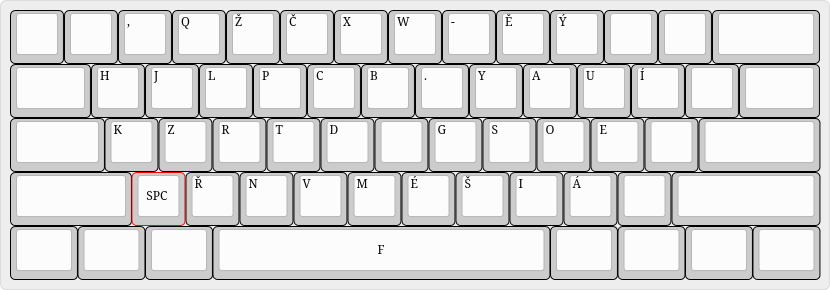
\includegraphics[width=\textwidth, height=0.8\textheight, keepaspectratio]{obrazky/hillclimb-1.png}
%    \caption{Výsledky prvního spuštění horolezeckého algoritmu}
%\end{figure}
\begin{figure}[h]
    \centering
    \caption{Výsledky prvního spuštění horolezeckého algoritmu}
    \vspace{0.5cm}
    \begin{keyboardlayout}
        % Row 1 (Numbers)
        \key{ }{1} \key{,}{1} \key{Q}{1} \key{Ž}{1} \key{Č}{1} \key{X}{1} \key{W}{1} \key{-}{1} \key{Ě}{1} \key{Ý}{1} \key{ }{1} \key{ }{1} \key{ }{1} \key{ }{2}
        \newrow
        % Row 2 (Tab)
        \key{ }{1.5} \key{H}{1} \key{J}{1} \key{L}{1} \key{P}{1} \key{C}{1} \key{B}{1} \key{.}{1} \key{Y}{1} \key{A}{1} \key{U}{1} \key{Í}{1} \key{ }{1} \key{ }{1.5}
        \newrow
        % Row 3 (Caps)
        \key{ }{1.75} \key{K}{1} \key{Z}{1} \key{R}{1} \key{T}{1} \key{D}{1} \key{G}{1} \key{S}{1} \key{O}{1} \key{E}{1} \key{ }{1} \key{ }{1} \key{ }{2.25}
        \newrow
        % Row 4 (Shift)
        \key{ }{2.25} \key{SPC}{1} \key{Ř}{1} \key{N}{1} \key{V}{1} \key{M}{1} \key{É}{1} \key{Š}{1} \key{I}{1} \key{Á}{1} \key{ }{1} \key{ }{2.75}
        \newrow
        % Row 5 (Space)
        \key{ }{1.25} \key{ }{1.25} \key{ }{1.25} \key{ }{6.25} \key{ }{1.25} \key{ }{1.25} \key{ }{1.25} \key{ }{1.25}
    \end{keyboardlayout}
    \small{Zdroj: Vlastní zpracování}
    \label{pic:hcwrong}
\end{figure}


Druhé spuštění tedy vyneslo zcela jiné výsledky, zejména hodnota nákladu
byla vyšší, a to $C_{Hill-2}=2,2677$. Nicméně při tomto spuštění byla vypozorována chyba 
v definici mapy klávesnice, jelikož ani jeden z výsledků nevyužíval fyzickou klávesu 
'H'. Proběhla oprava opětovné spuštění optimalizačního skriptu.

Třetí iterace horolezeckého algoritmu nabrala ještě nepatrně vyšší hodnotu nákladu 
$C_{Hill-3}=2,6855$ a výsledkem bylo rozložení klávesnice na obrázku \ref{pic:hcfinal}.
\begin{figure}[h]
    \centering
    \caption{Výsledky třetího spuštění horolezeckého algoritmu}
    \vspace{0.5cm}
    \begin{keyboardlayout}
        % Row 1 (Numbers)
        \key{ }{1} \key{ }{1} \key{W}{1} \key{É}{1} \key{Q}{1} \key{Ž}{1} \key{Ú}{1} \key{Š}{1} \key{Ů}{1} \key{Ý}{1} \key{X}{1} \key{ }{1} \key{ }{1} \key{ }{2}
        \newrow
        
        % Row 2 (Tab)
        \key{ }{1.5} \key{D}{1} \key{Ě}{1} \key{Z}{1} \key{Č}{1} \key{J}{1} \key{E}{1} \key{Ř}{1} \key{Y}{1} \key{A}{1} \key{.}{1} \key{K}{1} \key{ }{1} \key{ }{1.5}
        \newrow
        
        % Row 3 (Caps)
        \key{ }{1.75} \key{T}{1} \key{G}{1} \key{S}{1} \key{L}{1} \key{R}{1} \key{N}{1} \key{F}{1} \key{U}{1} \key{O}{1} \key{P}{1} \key{ }{1} \key{ }{2.25}
        \newrow
        
        % Row 4 (Shift)
        \key{ }{2.25} \key{B}{1} \key{Í}{1} \key{C}{1} \key{V}{1} \key{M}{1} \key{H}{1} \key{Á}{1} \key{I}{1} \key{,}{1} \key{ }{1} \key{ }{2.75}
        \newrow
        
        % Row 5 (Space)
        \key{ }{1.25} \key{ }{1.25} \key{ }{1.25} \key{ }{6.25} \key{ }{1.25} \key{ }{1.25} \key{ }{1.25} \key{ }{1.25}
    \end{keyboardlayout}
    \small{Zdroj: Vlastní zpracování}
    \label{pic:hcfinal}
\end{figure}
%\begin{figure}[h]
%    \centering
%    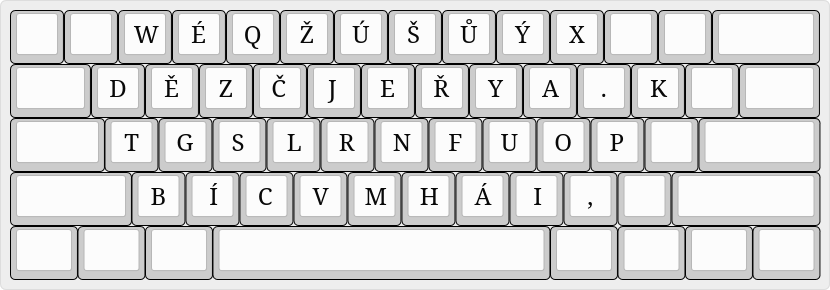
\includegraphics[width=\textwidth, height=0.8\textheight, keepaspectratio]{obrazky/hillclimb-3.png}
%    \caption{Výsledky třetího spuštění horolezeckého algoritmu}
%\end{figure}

Zajímavý je zde zejména shluk 'A', 'U', 'O' a 'I' na pravé straně klávesnice. Tyto samohlásky 
sice nejsou na domácí řadě, jak by se dalo předpokládat, nicméně jejich přilehlost 
vypovídá o jejich frekvenci výskytu. Dále je zajímavé, že klávesy 'C' a 'V' zůstávají 
na svých klasických pozicích. V poslední řadě stojí za zmínku posun klávesy ',' o 
jednu pozici doprava, což je jedna z nejnáročnějších změn z~hlediska svalové 
paměti.

\subsubsection{Horolezecký algoritmus s náhodnými restarty}
Před přesunem na simulované žíhání vznikl ještě jeden mezikrok, a to implementace
horolezeckého algoritmu s náhodným restartováním. Skript horolezeckého algoritmu 
byl upraven tak, aby optimalizační jádro skriptu bylo opakovaně spouštěno z náhodných 
startovních pozic. První spuštění tedy proběhlo klasicky z~QWERTZ rozložení, ale 
další iterace začínaly z náhodně vybraných map znaků vygenerovaných během realizace
horolezeckého algoritmu. Hodnota nákladové funkce 
každého cyklu algoritmu byla porovnána s předchozí nejnižší hodnotou. Nižší hodnota
z těchto dvou byla na konci cyklu nastavena jako nové minimum.

Pro první spuštění tohoto algoritmu bylo zvoleno 50 cyklů. Ve snaze snížit dobu 
zpracování tohoto úkolu bylo do skriptu implementováno paralelní zpracování 
na všech jádrech procesoru. Povaha algoritmu, kdy každý nový běh je 
nezávislý na výsledku předchozího běhu, je ideální pro implementaci paralelního 
zpracování. To je velká výhoda oproti algoritmu simulovaného žíhání, který musí 
sbíhat sekvenčně. Dokončení skriptu trvalo přes 16 minut a~výsledná 
hodnota nákladu $C_{RRHC}=2,6658$, což je značné zlepšení oproti běžnému 
hill climbing algoritmu, který se předvídatelně a prokazatelně zastavil v lokálním 
minimu, které je vyobrazeno na obrázku \ref{pic:rrhc}.

\begin{figure}[h!]
    \centering
    \caption{Výsledné rozložení horolezeckého algoritmu s náhodnými restarty}
    \vspace{0.5cm}
    \begin{keyboardlayout}
        % Row 1 (Numbers)
        \key{ }{1} \key{ }{1} \key{Ú}{1} \key{,}{1} \key{Ž}{1} \key{Q}{1} \key{Ý}{1} \key{X}{1} \key{Ů}{1} \key{W}{1} \key{Š}{1} \key{ }{1} \key{ }{1} \key{ }{2}
        \newrow
        
        % Row 2 (Tab)
        \key{ }{1.5} \key{R}{1} \key{B}{1} \key{Ř}{1} \key{D}{1} \key{P}{1} \key{E}{1} \key{Č}{1} \key{A}{1} \key{U}{1} \key{H}{1} \key{F}{1} \key{ }{1} \key{ }{1.5}
        \newrow
        
        % Row 3 (Caps)
        \key{ }{1.75} \key{N}{1} \key{K}{1} \key{.}{1} \key{T}{1} \key{L}{1} \key{É}{1} \key{G}{1} \key{O}{1} \key{I}{1} \key{S}{1} \key{ }{1} \key{ }{2.25}
        \newrow
        
        % Row 4 (Shift)
        \key{ }{2.25} \key{M}{1} \key{V}{1} \key{J}{1} \key{Z}{1} \key{C}{1} \key{É}{1} \key{Á}{1} \key{Í}{1} \key{Y}{1} \key{ }{1} \key{ }{2.75}
        \newrow
        
        % Row 5 (Space)
        \key{ }{1.25} \key{ }{1.25} \key{ }{1.25} \key{ }{6.25} \key{ }{1.25} \key{ }{1.25} \key{ }{1.25} \key{ }{1.25}
    \end{keyboardlayout}
    
    \small{Zdroj: Vlastní zpracování}
    \label{pic:rrhc}
\end{figure}

%\begin{figure}[h!]
%    \centering
%    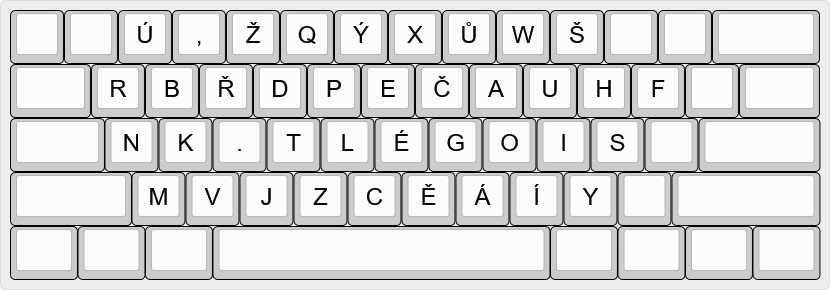
\includegraphics[width=\textwidth, height=0.8\textwidth, keepaspectratio]{obrazky/random-restart-hillclimb.png}
%    \caption{Výsledné rozložení horolezeckého algoritmu s náhodnými restarty}
%\end{figure}\footnote{Nevím proč se mi změnil font na obrázku, budu muset prozkoumat a předělat}

Z diagramu je vidět opět trend shlukování samohlásek k sobě do pravé části klávesnice. 
Dále je zajímavá poloha tečky na domovské řadě. Podobně jako tomu bylo v~předchozím výsledku 
se málo používané znaky jako 'Q', 'W' a 'X' přesou-vají do vrchní řady. Bylo by snadné usoudit,
že čím více se výsledek optimalizací přibližuje absolutnímu optimu, tím méně bude
rozdílů mezi výsledky, a zatímco lze pozorovat různé trendy (např. klávesy 'Q', 'W' a 'X' v horní řadě),
ještě je velká část klávesnice, která se vymyká pravidlům a pravděpodobně se bude dál vyvíjet 
a~měnit.

Vzhledem k závislosti algoritmu na náhodě jsou tyto výsledky špatně replikovatelné,
druhé spuštění skriptu bez jakýchkoliv úprav skončilo s vyšším nákladem
$C_{RRHC2}=2.6781$. Při dostatečném množství cyklů se teoreticky lze 
přiblížit globálnímu optimu, nicméně tento algoritmus je na hledání globálního 
optima časově náročný a výpočetně neefektivní.

\subsection{Aplikace algoritmu simulovaného žíhání}
Skript simulovaného žíhání velmi blízko kopíruje jeho teoretickou definici. 
Na začátku byly definovány parametry teploty a rychlosti chlazení. Pro první 
běh byla nastavena teplota $T=1$ a chlazení $\alpha=0,999$. Teplota, kdy algoritmus
končí, byla zvolena $T_{END}=0,00001$. Vzhledem k tomu, že 
hodnota $\alpha$ se blíží $1$, ochlazovaní probíhalo pomalu.

Algoritmus následně běží v cyklu, dokud se teplota nepřiblíží hodnotě výsledné 
teploty $T_{END}$. V každém cyklu vygeneruje novou mapu s pouze dvěma náhodnými 
změnami, spočítá jejich rozdíl základů, a lepší řešení vždy přijímá. Horší řešení
jsou přijímána v závislosti na výši teploty v daném cyklu. Čím déle algoritmus 
běží, tím je teplota a pravděpodobnost výběru horšího řešení nižší. Teplota se 
snižuje v~každém cyklu podle vzorce: 
\begin{equation*}
    T_{NOVA}=T_{STARA}\times\alpha
\end{equation*}

První spuštění SA algoritmu dosáhlo o stupeň horšího výsledku než RRHC, a~to 
$C_{SA1}=2,6675$. I přestože skript prošel 115 124 iterací, seběhl výrazně
rychleji než RRHC a dosáhl téměř identické hodnoty nákladu.

Zejména zajímavé na tomto řešení, které je vidět na obrázku \ref{pic:sa}, je postupný přesun znaků s diakritikou do spodní 
řady a~shluk samohlásek tentokrát na levé straně klávesnice. Nicméně trend 
samohlásek pod jednou rukou přetrvává. Samohlásky se v češtině málokdy vyskytují 
ve dvojicích, takže dává smysl, aby je psala jedna ruka, když hned následující 
znak velmi pravděpodobně bude psát druhá ruka. Interpunkční znaky jsou nově 
odsunuty do vrchní řady. Dále se na vrchu klávesnice nachází písmena z konce 
abecedy, tak jako tomu bylo v předcho\-zích řešeních.

\begin{figure}[h]
    \centering
    \caption{Výsledné rozložení vytvořené pomocí simulovaného žíhání}
    \vspace{0.5cm}
    \begin{keyboardlayout}
        % Row 1 (Numbers)
        \key{ }{1} \key{ }{1} \key{Ú}{1} \key{X}{1} \key{W}{1} \key{Ů}{1} \key{Ž}{1} \key{,}{1} \key{F}{1} \key{.}{1} \key{Q}{1} \key{ }{1} \key{ }{1} \key{ }{2}
        \newrow
        
        % Row 2 (Tab)
        \key{ }{1.5} \key{Í}{1} \key{H}{1} \key{Z}{1} \key{É}{1} \key{Á}{1} \key{E}{1} \key{J}{1} \key{L}{1} \key{R}{1} \key{P}{1} \key{B}{1} \key{ }{1} \key{ }{1.5}
        \newrow
        
        % Row 3 (Caps)
        \key{ }{1.75} \key{I}{1} \key{S}{1} \key{U}{1} \key{O}{1} \key{A}{1} \key{G}{1} \key{C}{1} \key{T}{1} \key{N}{1} \key{K}{1} \key{ }{1} \key{ }{2.25}
        \newrow
        
        % Row 4 (Shift)
        \key{ }{2.25} \key{Ý}{1} \key{Š}{1} \key{Č}{1} \key{Ě}{1} \key{Y}{1} \key{Ř}{1} \key{V}{1} \key{M}{1} \key{D}{1} \key{ }{1} \key{ }{2.75}
        \newrow
        
        % Row 5 (Space)
        \key{ }{1.25} \key{ }{1.25} \key{ }{1.25} \key{ }{6.25} \key{ }{1.25} \key{ }{1.25} \key{ }{1.25} \key{ }{1.25}
    \end{keyboardlayout}
    \small{Zdroj: Vlastní zpracování}
    \label{pic:sa}
\end{figure}

%\begin{figure}[h]
%    \centering
%    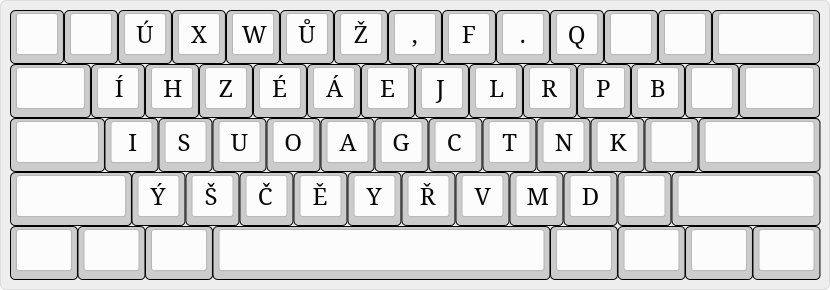
\includegraphics[width=\textwidth, height=0.8\textwidth, keepaspectratio]{obrazky/simulated-annealing.png}
%    \caption{Výsledné rozložení vytvořené pomocí simulovaného žíhání}
%\end{figure}



\subsection{Aplikace algoritmu optimalizace mravenčí kolonií}

Pro potřeby implementace byly nejprve stanoveny dva hlavní faktory. Heuristika ($\eta$)
počítá přitažlivost každé pozice pro každý znak ještě předtím, než se mravenci 
rozběhnou. Základní myšlenkou je, že nejčastěji použávaná písmena by měla být 
na nejlépe dostupných klávesách. Druhým faktorem jsou feromonoy ($\tau$). Na začátku 
algoritmu je všude stejné množství feromonů, a s postupným během algoritmu zanechávají 
mravenci, kteří postavili lepší klávesnici, více feromonů na použitých pozicích.

V každé generaci se rozběhne $n$ mravenců a každý z nich je postaven před prázdnou 
klávesnici. Každý mravenec následně dostane náhodně seřazený sez\-nam znaků. Jeden 
po druhém tyto znaky pokládaj na volné pozice podle s pravděpodob\-ností, 
která je určena podle vzorce $P = \tau^\alpha \times \eta^\beta$. V této rovnici 
je $\alpha$ váha feromonu a $\beta$ je váha heuristiky. Takto určenou pravděpodobností 
poskládají celou klávesnici.

Když všichni mravenci dostaví své klávesnice, jsou všechny ohodnoceny pod\-le hodnoty 
nákladu. Následuje odpařování feromonů, aby se mravenci nezasekli u prvního nejlepšího 
řešení, a zanechání nových feromonů. Poté startuje nová generace. Počet iterací 
je jeden ze vstupních parametrů a určuje, kdy algoritmus skončí.

Aplikace algoritmu optimalizace mravenčí kolonií na problém optimalizace rozložení
klávesnice měl horší výsledky než jaký byl předpoklad. Po 26 generacích se hodnota 
nákladu zastavila na $C_{ACO} = 3,6538$, což je překvapivě vysoká hodnota, zvlášť 
v porovnání se základním QWERTZ rozložením, které má hodnotu nákladu jen nepatrně 
vyšší ($C_{QWERTZ} = 3.7303$).

Po dalším přezkoumání bylo zjištěno, že ACO ve formě, ve které byl algoritmus 
implementován, je neefektivní pro tento problém. Jde především o stanovení základní 
nákladové funkce, která nastavuje váhu unigramů $\alpha = 0,2$ a trigramů 
$\gamma = 0,8$. Heuristika ACO algoritmu je v tomto případě stanovena jako 
\textit{Frekvence znaku / Náklad pozice}, což v praxi znamená, že mravenci agresivně 
optimalizují pro unigramy a vztahy mezi znaky téměř neřeší. Výsledkem tohoto 
algoritmu je následující rozložení:

\begin{figure}[h]
    \centering
    \caption{Výsledné rozložení původní verze ACO algoritmu}
    \vspace{0.5cm}
    \begin{keyboardlayout}
        % Row 1 (Numbers)
        \key{ }{1} \key{ }{1} \key{X}{1} \key{Ů}{1} \key{J}{1} \key{P}{1} \key{Z}{1} \key{Ž}{1} \key{D}{1} \key{Y}{1} \key{Q}{1} \key{ }{1} \key{ }{1} \key{ }{2}
        \newrow
        
        % Row 2 (Tab)
        \key{ }{1.5} \key{M}{1} \key{Í}{1} \key{R}{1} \key{Ř}{1} \key{Č}{1} \key{C}{1} \key{K}{1} \key{Ý}{1} \key{F}{1} \key{A}{1} \key{U}{1} \key{ }{1} \key{ }{1.5}
        \newrow
        
        % Row 3 (Caps)
        \key{ }{1.75} \key{.}{1} \key{S}{1} \key{Ú}{1} \key{T}{1} \key{N}{1} \key{B}{1} \key{H}{1} \key{É}{1} \key{I}{1} \key{V}{1} \key{ }{1} \key{ }{2.25}
        \newrow
        
        % Row 4 (Shift)
        \key{ }{2.25} \key{O}{1} \key{Ě}{1} \key{L}{1} \key{Á}{1} \key{G}{1} \key{,}{1} \key{W}{1} \key{Š}{1} \key{E}{1} \key{}{1} \key{ }{2.75}
        \newrow
        
        % Row 5 (Space)
        \key{ }{1.25} \key{ }{1.25} \key{ }{1.25} \key{ }{6.25} \key{ }{1.25} \key{ }{1.25} \key{ }{1.25} \key{ }{1.25}
    \end{keyboardlayout}
    \small{Zdroj: Vlastní zpracování}
    \label{pic:aco}
\end{figure}

I přestože je tento výsledek selháním v rámci širšiho kontextu, stejně je zajímavý.
Představuje totiž jednu z možných podob rozložení klávesnice, kdyby byla 
optimalizace zaměřena pouze na ideální pozici znaků a na pohodlí a rychlost 
psaní nebyl brán ohled.

\subsubsection{Úprava ACO na memetickou variantu}
Vzhledem k neuspokojivým výsledkům samostatné optimalizace mravenčí kolonií byl
optimalizační skript pro ACO upraven na memetickou variantu podle kapitoly 3.6.4.

Mravenci tedy fungují stejně jako v předchozí kapitole. Skládají klávesnici podle 
vzorce $P = \tau^\alpha \times \eta^\beta$. Tímto způsobem vytvoří „hrubý návrh“
který tedy vytvoří dobré rozložení pro izolované unigramy, ale není vhodný 
pro samotné psaní. Skript optimalizace mravenčí kolonií byl tedy rozšířen o funkci,
(get\_local\_search), která převezme rozložení klávesnice a následně na něm provádí 
algoritmus lokální\-ho prohledávání. Ten zkusí $n-$krát náhodně prohodit 2 klávesy.
Pokud prohození sníží celkovou námahu (sníží se hodnota nákladu), změnu ponechá.
%\footnote{co když sériově zlepší rozložení? sbíhá to natvrdo 40x nebo se zastaví po prvním zlepšení?}
Množství feromonů je následně převzato z nefinálního optimalizovaného řešení. Aplikuje se 
ale na cestu před optimalizací. Tímto způsobem je signalizováno mravencům, že jimi 
nalezené řešení je dobrý odrazový můstek pro další úpravy.

%Když mravenec staví klávesnici, umisťuje písmena jedno po druhém. Má sice heuristiku (ví, že 'E' %patří na dobré místo), ale nevidí souvislosti (trigramy). Může se stát, že sice položí 'S', 'C' a %'H' na ty nejlepší a nejdostupnější klávesy, ale nevšimne si, že je dal všechny na stejný prst, což %při psaní slova "schovat" vytvoří obrovskou ergonomickou penalizaci.%Tento hybridní skript to řeší následovně:%1. Hrubá stavba (Konstruktivní fáze)%Mravenec funguje úplně stejně jako minule. Pomocí rovnice P=τα⋅ηβ poskládá na základě heuristiky a %eromonů svou klávesnici. Vytvoří jakýsi "hrubý návrh", který má skvěle vyřešená častá písmena, %le pravděpodobně obsahuje skryté chyby v návaznostech (zlé trigramy).%. Učesání detailů (Hybridizace / Hill Climbing)tady přichází na řadu nová funkce quick_local_search. Hotový hrubý návrh mravence se předá tomuto "korektorovi". Ten zkusí 40krát náhodně prohodit dvě klávesy. Pokud prohození sníží celkovou námahu (například tím, že rozbije onen špatný shluk písmen S-C-H na jednom prstu), změnu si ponechá. Výsledkem je lokálně optimalizovaná, vyhlazená klávesnice.3. Odměňování a "Baldwinův efekt"
%Náklad (final_cost), ze kterého se počítá množství feromonu, se bere z vylepšené klávesnice.
%Feromon se ale sype na původní cestu (mapping), kterou vybral mravenec v kroku 1.
%Tento fenomén se v evolučních algoritmech nazývá Baldwinovské učení (na rozdíl od Lamarckovského, 
%kde by se feromony sypaly na upravenou cestu). Mravenec vlastně říká kolonii: "Tato hrubá stavba, 
%kterou jsem vymyslel, je vynikající odrazový můstek! Když začnete odsud, po pár drobných úpravách 
%získáte dokonalou klávesnici." 
%### Proč je to tak efektivní?
%Mravenci (ACO) zajistí, že algoritmus zkoumá slibné globální oblasti a nenechá se chytit v jedné 
%slepé uličce. Spolehlivě umístí nejdůležitější znaky.
%Hill Climbing zajistí precizní dotáhnutí detailů a zničí ergonomické "pasti", které by mravencům 
%trvalo desítky generací náhodně překonat.
%Spolu tak tvoří ideální balanc mezi průzkumem neznámého (exploration) a těžením z nalezeného (exploitation).

Po úpravě a spuštění bylo dosaženo $C_{M-ACO} = 3,1514$, což je výrazné zlepšení 
v porovnání s původní variantou algoritmu, nicméně opět jde o vysokou hodnotu a 
metoda optimalizace mravenčí kolonií se ukazuje jako spíše nevhodná pro problém 
optimalizace klávesnice. Výsledek je zobrazen na obrázku \ref{pic:maco}.

\begin{figure}[h]
    \centering
    \caption{Výsledek optimalizace pomocí M-ACO}
    \vspace{0.5cm}
    \begin{keyboardlayout}
        % Row 1 (Numbers)
        \key{ }{1} \key{ }{1} \key{Ů}{1} \key{H}{1} \key{Ú}{1} \key{X}{1} \key{Q}{1} \key{,}{1} \key{M}{1} \key{Ř}{1} \key{É}{1} \key{ }{1} \key{ }{1} \key{ }{2}
        \newrow
        
        % Row 2 (Tab)
        \key{ }{1.5} \key{N}{1} \key{Í}{1} \key{K}{1} \key{G}{1} \key{B}{1} \key{Š}{1} \key{Ý}{1} \key{Č}{1} \key{A}{1} \key{.}{1} \key{Ž}{1} \key{ }{1} \key{ }{1.5}
        \newrow
        
        % Row 3 (Caps)
        \key{ }{1.75} \key{L}{1} \key{E}{1} \key{Ě}{1} \key{P}{1} \key{T}{1} \key{J}{1} \key{Z}{1} \key{I}{1} \key{Á}{1} \key{Y}{1} \key{ }{1} \key{ }{2.25}
        \newrow
        
        % Row 4 (Shift)
        \key{ }{2.25} \key{F}{1} \key{U}{1} \key{R}{1} \key{D}{1} \key{C}{1} \key{V}{1} \key{W}{1} \key{O}{1} \key{S}{1} \key{}{1} \key{ }{2.75}
        \newrow
        
        % Row 5 (Space)
        \key{ }{1.25} \key{ }{1.25} \key{ }{1.25} \key{ }{6.25} \key{ }{1.25} \key{ }{1.25} \key{ }{1.25} \key{ }{1.25}
    \end{keyboardlayout}
    \small{Zdroj: Vlastní zpracování}
    \label{pic:maco}
\end{figure}

Tento výsledek je zajímavý oproti ostatním tím, že nedává samohlásky jen na 
domácí řadu. E a Ě jsou spolu s U a Í pod levou rukou, a písmena I, Á, A a O jsou
pod pravou rukou napříč všemi třemi základními řadami. Zajímavé je také přednost 
písmen W a Ž před písmeny H a M. První dvojice je na lépe dosažitelných pozicích 
než druhá dvojice, přestože se přirozeným odhadem může zdát, že H a M budou v~českých 
textech důležitější než W a Ž.

\subsection{Aplikace algoritmu optimalizace hejnem částic}
Pro potřeby optimalizace rozložení kláves na klávesnici nelze aplikovat základ\-ní 
verzi PSO algoritmu, jelikož optimalizace hejnem částic je navržena pro kontinuální 
prostory (\cite{pso-overview}, s. 12). Problém uspořádání klávesnice je ale diskrétní
kombinatorický problém, který je často modelovan jako kvadratický problém přiřaze\-ní 
(QAP) (\cite{Dey2024-nk}, s. 12). Pro účely této práce tedy byla využita hybridní 
varianta algoritmu, využívající kombinaci PSO a metody hill climbing. Tato implementace 
také využívá koncept prohození sekvencí, popsaný níže.
%Matematicky jde o bijektivní zobrazení množiny znaků na množinu fyzických kláves.

Každá částice vstupující do procesu reprezentuje jedno validní, náhodné rozlo\-žení klávesnice, 
ne bod v prostoru. Mechanismus pohybu je stanoven pozicí částic, vzdáleností a rychlostí.
Pozice udává konkrétní rozložení klávesnice, vzdálenost je seznam prohození, které 
jsou potřeba udělat, aby z rozložení A vzniklo rozložení B. Nakonec rychlost částic
je definována jako množina transpozic, které jsou nutné k transformaci aktuálního rozložení na nejlepší 
známé osobní řešení (pBest) a~globální řešení (gBest). 
Toto řešení bylo zvoleno, 
jelikož nelze jednoduše sčítat pozice písmen.

Na začátku algoritmu jsou stanoveny parametry, jde o počet částic, počet iterací,
učící faktory $C_1$ (kognitivní) a $C_2$ (sociální) a setrvačnost.
\begin{itemize}
    \item Kognitivní koeficient udává, jak moc je pohyb částice ovlivněn směrem k~pBest.
    \item Sociální koeficient určuje do jaké míry se částice pohybuje s davem k~Best.
    \item Setrvačnost stanovuje míru náhodného pohybu částice. V průběhu algoritmu se snižuje,
    tedy ze začátku je větší pravděpodobnost prozkoumání náhodného řešení a postupně se usazuje.
\end{itemize}

Pohyb částice spočívá v tom, že částice zkontroluje hodnotu svého 
nejlepšího řešení a hodnotu nejlepšího řešení celého hejna. Následně hledá možné 
transpozice směrem k pBest a gBest rozložení. Na základě pravděpodobnosti vycházející 
ze vstupních parametrů provádí vybrané transpozice. Součástí pohybu je hill climbing
pro urychlení lepších řešení. Bez této úpravy by částice mohly dlouho obíhat kolem 
lepších řešení.

Jádro algoritmu se skládá z inicializace (vytvoření částic) a hlavního cyklu. Ten 
pro každou částici spočítá náklad, aktualizuje globální nejlepší rozložení (pokud vzniklo),
vyvolá pohyb částic a sníží míru chaosu způsobenou vyšší hodnotou setrvačnosti.

Výsledkem prvního spuštění algoritmu je hodnota nákladové funkce $C_{PSO}=2,7029$ ze 
startovní pozice nákladu $C_{PSO-Start}=3,9001$.
Jde tedy o výrazně lepší výsledek, než jakého bylo dosaženo v předchozí kapitole, 
nicméně v porovnání s~předchozími řešeními, jako například s výsledkem simulovaného 
žíhání, jde stále o poměrně velkou hodnotu a výsledek je daleko od optimálního 
řešení.

Vzhledem k nedeterministké povaze algoritmu (startovní bod vychází z náho\-dy), druhé 
spuštění algoritmu startovalo na hodnotě $C_{PSO-Start-2}=3,8887$. Výsledná nákladová
funkce přinesla nepatrně lepší řešení $C_{PSO-2}=2,6804$.

Zvýšením počtu částic a prodloužením doby běhu algoritmu se ani po několi\-ka spuštěních 
nepodařilo snížit nákladovou funkci pod $2,6$. Výsledek optimalizace se 
40 částicemi po 100 generacích dosáhne nejlepšího výsledku ve .22 generaci, kdy 
náklad $C=2,6595$ a výsledné rozložení je na obrázku \ref{pic:pso}. Trend těchto optimalizací je jasný, nejnižší hodnoty nákladu bylo 
téměř vždy dosaženo mezi 20. a~35. generacemi, a hodnoty nákladu 
spadaly do intervalu $(2,8 : 2,65)$

\begin{figure}[h]
    
    \centering
    \caption{Výsledek optimalizace pomocí PSO}
    \vspace{0.5cm}
    \begin{keyboardlayout}
        % Row 1 (Numbers)
        \key{ }{1} \key{ }{1} \key{Ž}{1} \key{Ř}{1} \key{Č}{1} \key{Q}{1} \key{X}{1} \key{W}{1} \key{Š}{1} \key{Ú}{1} \key{Ů}{1} \key{ }{1} \key{ }{1} \key{ }{2}
        \newrow
        
        % Row 2 (Tab)
        \key{ }{1.5} \key{G}{1} \key{C}{1} \key{R}{1} \key{D}{1} \key{M}{1} \key{F}{1} \key{,}{1} \key{É}{1} \key{A}{1} \key{Y}{1} \key{U}{1} \key{ }{1} \key{ }{1.5}
        \newrow
        
        % Row 3 (Caps)
        \key{ }{1.75} \key{Z}{1} \key{T}{1} \key{N}{1} \key{K}{1} \key{ G}{1} \key{.}{1} \key{H}{1} \key{S}{1} \key{O}{1} \key{E}{1} \key{ }{1} \key{ }{2.25}
        \newrow
        
        % Row 4 (Shift)
        \key{ }{2.25} \key{Ě}{1} \key{J}{1} \key{L}{1} \key{B}{1} \key{P}{1} \key{I}{1} \key{Ý}{1} \key{Á}{1} \key{Í}{1} \key{}{1} \key{ }{2.75}
        \newrow
        
        % Row 5 (Space)
        \key{ }{1.25} \key{ }{1.25} \key{ }{1.25} \key{ }{6.25} \key{ }{1.25} \key{ }{1.25} \key{ }{1.25} \key{ }{1.25}
    \end{keyboardlayout}
    
    \small{Zdroj: Vlastní zpracování}
    \label{pic:pso}
\end{figure}


Na grafu \ref{graph:konvergence} je vidět, že nemá smysl zvyšovat počet generací algoritmu, jelikož 
skritp začne velmi brzy konvergovat k jeho finální hodnotě.

\begin{graph}[h!]
    \centering
    \caption{Znázornění konvergence PSO algoritmu}
    \vspace{0.5cm}
\begin{tikzpicture}
    \begin{axis}[
        %title={\textbf{Konvergence Hybridního PSO (40 částic)}},
        xlabel={Generace},
        ylabel={Nejlepší náklad (gBest)},
        grid=major,
        width=12cm,
        height=8cm,
        xmin=0, xmax=23, % Rozsah osy X
        ymin=2.6, ymax=4.0, % Rozsah osy Y
        legend pos=north east,
        cycle list name=color list,
        ylabel style={yshift=5pt},
        mark size=2pt
    ]

    \addplot+[
        thick,
        color=myblue,
        mark=*,
        mark options={fill=blue}
    ] coordinates {
        (0, 3.8839)
        (1, 3.0406)
        (2, 2.8659)
        (3, 2.7860)
        (4, 2.7191)
        (5, 2.7103)
        (6, 2.6944)
        (7, 2.6756)
        (8, 2.6716)
        (9, 2.6701)
        (10, 2.6691)
        (14, 2.6689)
        (15, 2.6607)
        (20, 2.6602)
        (21, 2.6601)
        (22, 2.6595)
    };
    \addlegendentry{gBest Cost}

    % Zvýraznění finálního bodu
    \node[pin={100:\textbf{2.6595}}, draw=black, circle, fill=red, inner sep=1pt] 
        at (axis cs:22, 2.6595) {};

    \end{axis}

    %\caption{Ukázka konvergence PSO k dané hodnotě}

    \end{tikzpicture}
    \label{graph:konvergence}
    
    \small{Zdroj: Vlastní zpracování}
\end{graph}

\subsection{Aplikace genetického algoritmu}
Největším problémem genetických algoritmů pro potřebu navržení nového rozložení 
klávesnice je permutace. Každé písmeno musí být na klávesnici právě jednou a žádné 
nesmí chybět. Kdyby bylo použito klasické jednobodové křížení, začnou vznikat neplatné 
děti (například klávesnice, na které je písmeno A dvakrát, ale E chybí). Aby se předešlo 
této chybě, vznikl algoritmus s využitím metody pořádkového křížení (anglicky order 
crossover, zkratka OX).

Pro zjednodušení skriptu je klávesnice převedena na jednodimenzionální sez\-nam znaků a jejich pozic.
Následně skript náhodně vybírá výsek znaků. Tyto znaky si dítě vezme od prvního rodiče a~umístí
je přesně na tytéž pozice. Tyto klávesy se označují jako obsazené. Zbylé znaky, 
které ještě nemají své místo, se musí rozdělit na volné klávesy. Algoritmus 
bere ze druhého rodiče volné klávesy přesně v takovém prostorovém pořadí, jaké preferuje
druhý rodič. Dítě tedy získalo část přesné struktury od prvního rodiče a část
ergonomické logiky (pořadí) od druhého rodiče, aniž by vznikl jakýkoliv duplikát.

Algoritmus následně simuluje skutečnou Darwinovskou evoluci tradičním způ\-sobem.
Skript nevybírá rodiče čistě podle toho absolutně nejlepšího, namísto toho bere pět náhodných 
klávesnic z populace a srovnává je mezi sebou. Vítěz s~nejnižším nákladem se stává rodičem.
Tento postup zachovává genetickou diverzitu a zabraňuje předčasné konvergenci. 

Dítě vzníklé pomocí OX má parametrem danou šanci, že u něj dojde k náhodné chybě v DNA 
(dojde k změně poloh dvou znaků). Mutace je nezbytná pro objevování úplně nových kombinací.

Nově zmutované dítě je podrobeno funkci lokálního hledání. Dítě sice získá genetické predispozice
od rodičů, ale předtím, než je zařazeno do nové generace, prochází lokálním hledáním pro 
opravu některých hrubých ergonomických chyb.

Nakonec, aby algoritmus neztratil v procesu křížení nejlepší řešení, dva absolutně 
nejlepší jedinci z každé generace jsou automaticky zkopírováni do další generace bez
jakéhokoliv křížení a mutací.

Nově vzniklé rozložení, s nákladovou hodnotou $C_{GA}=2,6195$. Jde tedy o nejlepší 
řešení, kterého bylo dosáhnuto. Nově vzniklé rozložení je popsáno na obráz\-ku číslo \ref{fig:GA-layout} 
a bude použito pro testování na fyzickém prototypu klávesnice.

\begin{figure}[H]
    
    \centering
    \caption{Výsledek optimalizace pomocí genetického algoritmu}
    \vspace{0.5cm}
    \begin{keyboardlayout}
        % Row 1 (Numbers)
        \key{ }{1} \key{ }{1} \key{,}{1} \key{Q}{1} \key{Ž}{1} \key{Ř}{1} \key{X}{1} \key{Ú}{1} \key{Ů}{1} \key{Ě}{1} \key{W}{1} \key{ }{1} \key{ }{1} \key{ }{2}
        \newrow
        
        % Row 2 (Tab)
        \key{ }{1.5} \key{D}{1} \key{C}{1} \key{B}{1} \key{J}{1} \key{L}{1} \key{V}{1} \key{Ý}{1} \key{I}{1} \key{A}{1} \key{U}{1} \key{Y}{1} \key{ }{1} \key{ }{1.5}
        \newrow
        
        % Row 3 (Caps)
        \key{ }{1.75} \key{T}{1} \key{G}{1} \key{K}{1} \key{R}{1} \key{N}{1} \key{S}{1} \key{Š}{1} \key{Í}{1} \key{O}{1} \key{F}{1} \key{ }{1} \key{ }{2.25}
        \newrow
        
        % Row 4 (Shift)
        \key{ }{2.25} \key{H}{1} \key{Č}{1} \key{P}{1} \key{M}{1} \key{Z}{1} \key{.}{1} \key{E}{1} \key{Á}{1} \key{É}{1} \key{}{1} \key{ }{2.75}
        \newrow
        
        % Row 5 (Space)
        \key{ }{1.25} \key{ }{1.25} \key{ }{1.25} \key{ }{6.25} \key{ }{1.25} \key{ }{1.25} \key{ }{1.25} \key{ }{1.25}
    \end{keyboardlayout}
    \small{Zdroj: Vlastní zpracování}
    \label{fig:GA-layout}
\end{figure}

I tento výsledek potvrzuje již výše popsané trendy. Samohlásky pod jednou rukou,
písmena málo používaná v českém jazyce na vrchní řadě a samohlásky s~diakritikou 
jsou blízko samohláskám bez diakritiky.

\subsection{Hardwarová implementace}
Pro možnost přesného měření kognitivní zátěže a rychlosti psaní bylo nutné 
optimalizované rozložení z genetického algoritmu implementovat do fyzického 
testovacího prototypu. Jako hardwarová platforma byla zvolena kompaktní kláves\-nice 
formátu 60 \% (model Unix60), konfigurovaná v rozložení vycházejícím ze standardu 
HHKB (Happy Hacking Keyboard). Cílem této implementace bylo vytvořit nezávislé 
vstupní zařízení (HID), které zpracovává mapování znaků přímo na úrovni vlastního 
mikrokontroléru bez nutnosti softwarových úprav v operačním systému hostitelského 
počítače.

Základní myšlenkou open-source firmwaru QMK (a jeho konfigurační nadstavby Vial) 
je práce s virtuálními vrstvami. Tyto vrstvy fungují na principu překrývajících 
se logických matic. Výchozí vrstva (Layer 0) byla ponechána se standardním 
rozložením QWERTZ. Optimalizované rozložení vygenerované genetickým algoritmem 
bylo implementováno jako dedikovaná samostatná vrstva (Layer 1). Klávesy, jejichž 
pozice nebyla algoritmem modifikována (např. mezerník, funkční klávesy a modifikátory), 
byly na vrstvě 1 definovány jako transparentní (KC\_TRNS), což zajišťuje propadnutí 
signálu do výchozí vrstvy a šetří paměť mikrokontroleru klávesnice.

Klíčovým prvkem uživatelského rozhraní pro plynulé přepínání mezi testovaným 
a~výchozím rozložením je využití pokročilé firmwarové funkce Tap Dance. Z hlediska 
softwarové architektury se jedná o implementaci konečného stavového automatu 
(Finite State Machine), který vyhodnocuje časová okna úhozů, v tomto případě 200 ms.

Tato logika byla namapována na klávesu levého modifikátoru Alt (LALT), situovanou 
bezprostředně vlevo od klávesy mezerníku. Volba této pozice je ergonomická, neboť 
umožňuje obsluhu silným palcem bez nutnosti vychýlení ruky ze základní pozice. 
Stavový automat rozlišuje tři základní scénáře:
\begin{enumerate}
    \item \textbf{Stisk a držení} (Hold): Mikrokontrolér odesílá standardní HID kód modifikátoru Alt.
    \item \textbf{Jeden krátký stisk} (Single Tap): Systém vyhodnotí úhoz jako standardní stisk klávesy Alt.
    \item \textbf{Rychlý dvojstisk} (Double Tap): Pokud systém detekuje dva úhozy v rámci 
    definovaného časového limitu, přejde do stavu Layer Toggle. Tento stav uzamkne 
    klávesnici v optimalizované vrstvě GA (Layer 1). Opětovný dvojitý stisk klávesy 
    LALT vyvolá inverzní funkci a vrátí uživatelské rozhraní do výchozího stavu 
    QWERTZ (Layer 0).
\end{enumerate}

\clearpage

\section{Zhodnocení výsledků}
Tato kapitola syntetizuje a kriticky zhodnocuje poznatky získané během 
optimalizačního procesu popsaného v předchozí části práce. Zatímco praktická 
část se soustředila primárně na technickou implementaci a běh vybraných 
heuristických algoritmů, cílem této kapitoly je analyzovat dosažené výsledky 
v širším kontextu ergonomie a praktické použitelnosti pro český jazyk.

V první části je provedena kvantitativní komparace výkonnosti jednotlivých 
algoritmů na základě hodnoty nákladové funkce a výpočetní náročnosti. Následně 
jsou vygenerovaná rozložení podrobena kvalitativní analýze z hlediska 
lingvistických a anatomických specifik, s důrazem na identifikaci společných 
trendů a~anomálií. Závěr kapitoly je věnován praktické validaci nejlepšího 
dosaženého řešení. Toto rozložení bylo naprogramováno do firmwaru fyzického 
prototypu klávesnice a otestováno pomocí standardizovaného měření, což 
umožňuje konfrontovat teoretické matematické modely s reálnou uživatelskou 
zkušeností a diskutovat tzv. produkční paradox.

\subsection{Srovnání výkonnosti optimalizačních algoritmů}
Graf \ref{graph:sronvani_algo} znázorňuje srovnání dosažených hodnot nákladové funkce pro jednotlivé 
testované algoritmy. Z výsledků je patrné, že nejlepších (nejnižších) hodnot 
dosáhla řešení založená na genetickém algoritmu (GA) a optimalizaci hejnem částic (PSO).
Nicméně mezi genetickým algoritmem, optimalizací hejnem částic, simulovaném žíháním (SA) 
a oběma metodami horolezeckého algoritmu (HC pro klasickou verzi a RRHC pro úpravu 
s náhodnými restarty) není výsledná hodnota nákladové funkce výrazně rozdílná.
Základní heuristika QWERTZ vykazuje nejvyšší nákladovost. Mezi QWERTZ a funkčními 
optimalizacemi se nachází obě použité varianty optimalizace mravenčí kolonií, tedy 
standardní ACO a memetická verze M-ACO, která díky úpravě dosáhla o 14 \% 
lepších výsledků než základní verze.

Navzdory předpokladům o vysoké schopnosti algoritmů mravenčí 
kolonie do\-sáhla ACO metoda při řešení tohoto konkrétního kombinatorického problému
vý\-razně horších výsledků. 
Hlavní příčinou selhání je brzká náchylnost této metody k uvíznutí v 
lokálním optimu. Hlavní výzvou těchto metaheuristických algoritmů je správné vyvažování 
parametrů, které zajistí průzkum nových oblastí a~zároveň vytěžování již nalezených 
slibných řešení (anglicky exploitation) (\cite{pso-overview}, s. 5; \cite{Dey2024-nk}, s. 133).


\begin{graph}[h!]
    \centering
    \caption{Srovnání algoritmů podle nákladové funkce}
    \vspace{0.5cm}
\begin{tikzpicture}
\begin{axis}[
    ybar,
    enlarge x limits=0.15,
    legend style={at={(0.5,-0.15)}, anchor=north, legend columns=-1},
    ylabel={Hodnota nákladové funkce},
    yticklabel style={
        /pgf/number format/fixed,
        /pgf/number format/precision=0
    },
    symbolic x coords={GA, PSO, RRHC, SA, HC, M-ACO, ACO, QWERTZ},
    xtick=data,
    nodes near coords,
    /pgf/number format/.cd,
    fixed,
    fixed zerofill, % doplní nuly, aby měly všechny popisky stejnou délku
    precision=3,    % počet desetinných míst
    use comma,      % vypíše čárku místo tečky
    /tikz/.cd,      % návrat do tikz na
    nodes near coords align={vertical},
    x tick label style={rotate=45, anchor=north east},
    width=12cm,
    height=8cm,
    bar width=20pt,
    grid=major,
    grid style={dashed, gray!30},
    %title={Srovnání algoritmů podle nákladové funkce},
    ymin=0,
    ymax=4.5, % Upraveno pro prostor nad popisky
]

\addplot[fill=myblue, draw=black!70, /pgf/number format/read comma as period] coordinates {
    (GA, 2,6195)
    (PSO, 2,6595)
    (RRHC, 2,6658)
    (SA, 2,6675)
    (HC, 2,6855)
    (M-ACO, 3,1514)
    (ACO, 3,6538)
    (QWERTZ, 3,7303)
};

\end{axis}
\end{tikzpicture}

    \label{graph:sronvani_algo}
    \small{Zdroj: Vlastní zpracování}
\end{graph}

%Wang a kol. (\cite{pso-overview}, s. 4-16) považuje tendenci uvíznout v lokálním optimu 
%za jednu z hlavních nevýhod algoritmu optimalizace hejnem částic, a to zejména u 
%funkcí, které mají mnoho lokálních extrémů. Hlavní příčinou je to, že rozmanitost 
%populace částic může velmi rychle zmizet. Jakmile jedna částice narazí na lokální 
%optimum, ostatní částice jsou k tomuto bodu silně přirahovány. Rychlé shlukování 
%částic do jednoho bodz následně způsobuje ztrátu schopnosti efektivně prozkoumávat 
%širší stavový prostor a algoritmus předčasně konverguje, aniž by nalezl globální 
%optimum. Navíc diskrétní verze PSO (pracující s celočíselnými nebo binárními 
%proměnnými) mají tendenci uvíznutí ještě výraznější. Ke zmírnění tohoto problému
%lze využít různé mechanismy, jako například přidání mutací (po vzoru genetických
%algoritmů) nebo odhánění částic od nejhorších nalezených řešení (takzvané negativní 
%posilování, anglicky negative reinforcement).

Potíže zasekávat se v lokálních optimech jsou u ACO především u problémů velkého 
rozsahu nebo u problémů s velmi členitým a složitým 
prostorem řešení (tzv. rugged landcscapes) (\cite{Dey2024-nk}, s. 71, 184). V~kontextu mravenčí kolonie se uvíznutí 
v lokálním optimu označuje jako stagnace (\cite{Dey2024-nk}, s. 25). 

Pérez-Carabaza a kol. (\cite{Dey2024-nk}, s. 19-44) udávají, že tento jev vzniká 
jako důsledek příliš 
silné zpětné vazby. Jakmile určitá cesta (i suboptimální) nahromadí mírně vyšší 
množství feromonu, přiláká více mravenců. To vede k dalšímu posílení této cesty, až 
nakonec všichni mravenci začnou sledovat tuto jedinou, identickou trasu. Jakmile 
tento stav stagnace nastane, prozkoumávání nových a potenciálně lepších řešení 
je zastaveno a algoritmus ztrácí schopnost uniknout z lokálního minima. 
Aby se 
předešlo uvíznutí v lokálním optimu, byly vyvinuty pokročilé varianty algoritmu. 
Například varianta Max-Min ant system to řeší tak, že zavádí přísné minimální a maximální
limity pro množství feromonu na jednotlivých hranách. Díky tomu žádná cesta nezeslábne
na nulu a žádná nezíská takovou dominanci, aby ji mravenci museli sledovat na 100\space\%.

Dalším možným řešením je cílené přidání prvků náhodnosti do rozhodování mravenců
(\cite{Dey2024-nk}, s. 71).

Z naměřených dat je patrné, že metody lokálního prohledávání (RRHC, SA) i~evoluční 
techniky (GA) konvergovaly k velmi podobným hodnotám nákladové funkce v intervalu 
$\langle 2,6195 - 2,6855 \rangle $. Tento jev indikuje vysoce členitý prostor řešení (tzv. fitness 
landscape) problému uspořádání klávesnice, který obsahuje obrovské množství 
lokálních minim s téměř identickou hodnotou nákladové funkce. Tento jev plně 
koresponduje s teorémem no free lunch, který postuluje, že pro množinu všech 
možných optimalizačních problémů neexistuje žádný univerzálně nadřazený 
algoritmus. Ukazuje se tedy, že žádná z testovaných metaheuristik nedokáže v~tomto 
specifickém prostoru absolutně dominovat, avšak všechny spolehlivě nacházejí řešení 
výrazně převyšující standard QWERTZ.

Přestože jsou rozdíly na této hranici minimální, absolutního optima v rámci 
realizovaných experimentů dosáhl genetický algoritmus s hodnotou nákladové funkce
$C_{GA}=2,6195$. Z tohoto důvodu bylo právě toto rozložení vybráno pro následnou 
detailní analýzu a praktické testování.
Jednotlivě se sice algoritmy signifikantně lišily ve své výpočetní náročnosti 
(např. běh genetického algoritmu trval řádově déle než rychlá konvergence 
simulovaného žíhání), avšak tento faktor nebyl při finální komparaci zohledněn. 
Vzhledem k povaze problému, který představuje jednorázovou optimalizaci, je pro 
praktické využití klíčová výhradně ergonomická kvalita nalezeného řešení, nikoliv 
čas potřebný k jeho vygenerování.
\subsubsection{Srovnání s ostatními standardními rozloženími}
Pro validaci přínosu navrženého řešení bylo vítězné rozložení (GA) srovnáno 
nejen s výchozím standardem QWERTZ, ale také s celosvětově nejrozšířenějšími 
alternativními rozloženími Dvorak a Colemak. Pro srovnání byly využity původní 
verze obou alternativních rozložení bez dalších úprav.

Z výsledků nákladové funkce (viz graf \ref{graph:global_comparison}) je však patrné, že efektivita těchto 
standardů je při aplikaci na český textový korpus omezená. Rozložení Dvorak 
vykázalo hodnotu nákladu 3,5379, což představuje pouze marginální zlepšení oproti 
QWERTZ. Rozložení Colemak dosáhlo lepších výsledků (3,3472), nicméně stále vykazuje 
o 25\space\% vyšší ergonomickou zátěž než rozložení vygenerované genetickým algoritmem (2,6195).

\begin{graph}[h!]
    \centering
    \caption{Srovnání optimalizovaného rozložení s globálními standardy}
    \vspace{0.5cm}
    \begin{tikzpicture}
    \begin{axis}[
        ybar,
        enlarge x limits=0.25,
        ylabel={Hodnota nákladové funkce},
        symbolic x coords={GA, Colemak, Dvorak, QWERTZ},
        xtick=data,
        nodes near coords,
        nodes near coords style={/pgf/number format/fixed, /pgf/number format/precision=4, font=\footnotesize},
        width=10cm,
        height=7.5cm,
        bar width=25pt,
        grid=major,
        grid style={dashed, gray!30},
        %title={Rozložení klávesnic},
        ymin=0, ymax=4.5,
    ]

    \addplot[fill=myblue, draw=black!80] coordinates {
        (GA, 2.6195)
        (Colemak, 3.3472)
        (Dvorak, 3.5379)
        (QWERTZ, 3.7303)
    };

    \end{axis}
    \end{tikzpicture}
    
    \label{graph:global_comparison}
    \small{Zdroj: Vlastní zpracování}
\end{graph}

Tato komparace dokazuje, že obecná ergonomická rozložení nejsou plně 
pře\-nositelná mezi jazyky s odlišnou fonetickou a lexikální strukturou. Zatímco 
mezinárodní standardy selhávají v efektivním mapování n-gramů 
a diakritiky, specifických pro české texty, navržený algoritmus adaptoval řešení přímo na míru 
českému jazyku. Tímto bylo dosaženo výrazně vyšší míry optimalizace než rozlo\-žení Colemak.

\subsection{Analýza vítězného rozložení}
Detailní kvalitativní analýza vítězného rozložení vygenerovaného genetickým algoritmem 
(Obrázek \ref{fig:GA-layout}) odhaluje logiku, kterou metaheuristika zvolila pro minimalizaci 
anatomické zátěže. Přestože se výsledná matice znaků na první pohled jeví jako 
neuspořádaná, z hlediska n-gramové frekvence a definované nákladové funkce 
představuje vysoce optimalizovaný systém postavený na dvou klíčových principech.

Prvním a výraznějším trendem je striktní rozdělení práce mezi levou a~pravou 
ruku (tzv. hand alternation). Algoritmus systematicky přesunul frekventované 
souhlásky (T, G, K, R, N, S atd.) na levý segment klávesnice, zatímco pravý 
segment byl vyhrazen primárně pro samohlásky a jejich varianty s~dlouze znějící 
diakritikou (A, E, I, O, U, Y, Á, É, Í). Vzhledem k fonetické struktuře českého 
jazyka, kde se nejčastěji střídají souhlásky a samohlásky, toto rozložení 
teoreticky maximalizuje plynulé střídání levé a pravé ruky při tvorbě běžných 
slabik a slov.

Druhým specifikem je vertikální rozprostření samohlásek na pravé straně. Na 
rozdíl od tradičních ergonomických rozložení (např. Dvorak), která umisťují 
samohlásky lineárně na domovskou řadu, GA využil všechny tři základní řady. Toto 
rozhodnutí je přímým důsledkem trigramové nákladové funkce, která silně penalizuje 
opakované použití stejného prstu. Vertikální distribuce zajišťuje, 
že při výskytu dvou samohlásek bezprostředně po sobě (např. dvojhlásky „ou“, „au“) 
dochází k plynulému zapojení různých prstů pravé ruky.

Diakritické znaky s nízkou frekvencí výskytu (Ž, Ř, Ů, Ě), společně s písmeny, které 
se v češtině příliš nevyužívají (Q, W, X), algoritmus odsunul na obtížně dosažitelnou 
číselnou řadu. Tím 
se uvolnil prostor v ergonomicky přívětivějších zónách (domovská a~horní řada) pro 
klíčové české n-gramy, což ospravedlňuje matematickou efektivitu tohoto uspořádání.

Pro objektivní evaluaci ergonomických přínosů optimalizovaného rozložení z~genetického 
algoritmu (GA) byla provedena analytická komparace statické zátě\-že s referenčním 
rozložením QWERTZ. Výpočet vycházel z relativní frekvence unigramů v korpusu české 
Wikipedie, přičemž pro zachování vypovídací hodnoty o~pohybu prstů nebyla do výpočtu 
zahrnuta klávesa mezerníku, jejíž pozice a~funkce (ovládání palci) zůstala u obou 
rozložení fixní.

V odborné literatuře se často zmiňuje ergonomický deficit rozložení QWERTY spočívající
ve výrazném přetěžování levé ruky, která dle analýz anglických textů vykonává až 57\space\% 
veškerých úhozů (\cite{qwerty-dilemma}, s. 1233; \cite{qwerty-immortal}, s. 118). 
Výsledky provedené frekvenční analýzy na českém korpusu však tento předpoklad pro 
českou lokalizaci QWERTZ vyvracejí. Jak ilustruje graf \ref{graph:balance_rukou}, 
uspořádání QWERTZ je při psaní českých textů téměř dokonale symetrické, s podílem 
40,7\space\% úhozů pro levou ruku a~41,4\space\% pro pravou ruku. Genetický algoritmus tuto 
existující makro-rovnováhu přirozeně zachoval (41,3\space\% ku 40,8\space\%).

\begin{graph}[h!]
    \centering
    \caption{Srovnání vyváženosti zátěže rukou u rozložení QWERTY a GA}
    \vspace{0.5cm}
    \begin{tikzpicture}
    \begin{axis}[
        ybar,
        enlarge x limits=0.4,
        ylabel={Podíl na psaní [\%]},
        symbolic x coords={QWERTY, GA},
        xtick=data,
        nodes near coords,
        nodes near coords style={/pgf/number format/fixed, /pgf/number format/precision=1},
        every node near coord/.append style={font=\footnotesize},
        legend style={at={(0.5,-0.2)}, anchor=north, legend columns=-1},
        width=10cm,
        height=6cm,
        bar width=20pt,
        grid=major,
        grid style={dashed, gray!30},
        % KLÍČOVÉ NASTAVENÍ: Zkrácení osy Y pro zvýraznění rozdílu
        ymin=47, 
        ymax=50, 
        ytick={47, 47.5, 48, 48.5, 49, 49.5, 50},
        extra y ticks={50},
        %extra y tick style={grid=major, grid style={thick, dashed}, tick label style={font=\footnotesize}},
        %extra y tick labels={Ideál (50\%)},
    ]

    % Levá ruka
    \addplot[fill=blue!60, draw=black!70] coordinates {
        (QWERTY, 48.3)
        (GA, 49.0)
    };

    % Pravá ruka
    \addplot[fill=orange!70, draw=black!70] coordinates {
        (QWERTY, 49.1)
        (GA, 48.4)
    };

    \legend{Levá ruka, Pravá ruka}
    \end{axis}
    \end{tikzpicture}
    
    \label{graph:balance_rukou}
    \small{Zdroj: Vlastní zpracování}
\end{graph}

Hlavní přínos optimalizace se tak projevil na úrovni mikropohybů a redistribuce 
zátěže mezi jednotlivými prsty. Z dat vizualizovaných na grafu \ref{graph:finger_load} 
je patrný cílený přesun zátěže na silnější 
a obratnější prsty, primárně na ukazováčky. Například zátěž levého ukazováčku 
vzrostla z 16,52\space\% u QWERTZ na 19,24\space\% u GA rozložení. Současně došlo k výrazné 
úlevě pro levý malíček, jehož zátěž klesla z téměř 12\space\% na pouhých 7\space\%.
\begin{graph}[hp]
    \centering
    \caption{Srovnání relativního vytížení jednotlivých prstů}
    \vspace{0.4cm}
    \begin{tikzpicture}
    \begin{axis}[
        ybar,
        bar width=7pt, % Užší sloupce, aby se jich tam vešlo 16
        width=14cm,    % Širší graf pro lepší čitelnost prstů
        height=7cm,
        ylabel={Zátěž prstů [\%]},
        symbolic x coords={L_R, L_P, L_M, L_I, P_I, P_M, P_P, P_R},
        xtick=data,
        xticklabels={Malíček L, Prsteník L, Prostředník L, Ukazovák L, Ukazovák P, Prostředník P, Prsteník P, Malíček P},
        x tick label style={rotate=45, anchor=north east, font=\small},
        nodes near coords,
        every node near coord/.append style={rotate=90, anchor=west, font=\tiny, /pgf/number format/fixed, /pgf/number format/precision=1},
        legend style={at={(0.5,-0.4)}, anchor=north, legend columns=-1},
        grid=major,
        grid style={dashed, gray!30},
        ymin=0, ymax=30, % Prostor pro popisky nad sloupci
    ]

    % DATA: ZÁKLADNÍ QWERTZ
    \addplot[fill=gray!40, draw=black!80] coordinates {
        (L_R, 5.66) (L_P, 8.93) (L_M, 14.14) (L_I, 19.59) 
        (P_I, 15.29) (P_M, 12.98) (P_P, 5.63) (P_R, 15.21)
    };

    % DATA: GA OPTIMALIZOVANÁ
    \addplot[fill=myblue, draw=black!80] coordinates {
        (L_R, 5.99) (L_P, 11.82) (L_M, 8.35) (L_I, 22.82) 
        (P_I, 9.65) (P_M, 15.43) (P_P, 6.06) (P_R, 17.30)
    };

    \legend{QWERTZ (Základní), GA (Optimalizovaná)}
    \end{axis}
    \end{tikzpicture}
    
    \label{graph:finger_load}
    \small{Zdroj: Vlastní zpracování}

    %\vspace{0.8cm}
    \caption{Srovnání zátěže jednotlivých řad}
    \vspace{0.4cm}
    \begin{tikzpicture}
    \begin{axis}[
        ybar,
        enlarge x limits=0.25,
        ylabel={Zátěž řad [\%]},
        symbolic x coords={N, H, M, D},
        xtick=data,
        xticklabels={Numerická (4.), Horní (3.), Domácí (2.), Dolní (1.)},
        x tick label style={font=\small},
        nodes near coords,
        nodes near coords style={/pgf/number format/fixed, /pgf/number format/precision=1, font=\footnotesize},
        width=12cm,
        height=8cm,
        bar width=22pt,
        grid=major,
        grid style={dashed, gray!30},
        legend style={at={(0.5,-0.15)}, anchor=north, legend columns=-1},
        %title={Srovnání vertikálního vytížení řad klávesnice},
        ymin=0, ymax=45,
    ]

    % DATA: ZÁKLADNÍ QWERTZ
    \addplot[fill=gray!40, draw=black!80] coordinates {
        (N, 8.98) (H, 37.88) (M, 29.23) (D, 21.34)
    };

    % DATA: GA OPTIMALIZOVANÁ
    \addplot[fill=myblue, draw=black!80] coordinates {
        (N, 3.85) (H, 33.03) (M, 37.24) (D, 23.30)
    };

    \legend{QWERTZ (Základní), GA (Optimalizovaná)}
    \end{axis}
    \end{tikzpicture}
    
    \label{graph:row_load}
    \small{Zdroj: Vlastní zpracování}
\end{graph}


Nejvýraznější kvalitativní posun však odhalila analýza využití jednotlivých 
horizontálních řad (numerická, horní, domovská, dolní). Graf \ref{graph:row_load} 
demonstruje zásad\-ní strukturální vadu uspořádání QWERTZ, které uživatele nutí 
nejčastěji operovat v~horní řadě (37,88\space\% úhozů), zatímco ergonomicky nejvýhodnější 
domovská řada (home row) je využita pouze z 29,23\space\%. V novém rozložení je tedy 
domácí řada využívána o 25\space\% více než při psaní v českém jazyce na QWERTZ klávesnici.


Optimalizace pomocí genetického algoritmu tento nepříznivý stav prokazatelně 
invertovala. Těžiště psaní bylo úspěšně přesunuto na domovskou řadu, která na 
novém rozložení absorbuje 37,24 \% veškeré zátěže (absolutní nárůst o 8\space\%). 
Obzvláště výrazným ergonomickým benefitem je pak drastická redukce úhozů směřujících 
do nejhůře dostupné numerické řady. Zatímco u QWERTZ vyžaduje natažení prstů do 
této krajní pozice téměř každý desátý úhoz (8,98\space\%), u~rozložení vygenerovaného 
pomocí genetického algoritmu klesla nutnost 
opustit standardní zónu dosahu na marginálních 3,85\space\%.

\subsection{Validace}
%Pro ověření praktické použitelnosti vygenerovaného rozložení byl sestrojen plně 
%funkční hardwarový prototyp s firmwarem QMK. Testování probíhalo na platformě 
%Monkeytype s využitím rozšířeného českého slovníku obsahujícího diakritiku a 
%interpunkci. Jako referenční hodnota (baseline) byl změřen průměrný výkon na 
%standardním rozložení QWERTZ, který činil X WPM s přesností Y \%. Následně 
%probíhala fáze adaptace na optimalizované rozložení v celkové délce Z hodin. 
%Výsledky měření ukázaly\dots

%Z hlediska limitů tohoto výzkumu je nutné uvést, že algoritmy inteligence hejna 
%(PSO) a mravenčí kolonie (ACO) byly implementovány s doporučeným výchozím 
%nastavením hyperparametrů. Ačkoliv by rozsáhlý fine-tuning (např. detailní 
%kalibrace kognitivních a sociálních koeficientů u PSO) mohl vést k dílčímu 
%snížení hodnoty nákladové funkce, pro účely této práce nebyl realizován. 
%Důvodem je skutečnost, že u těchto algoritmů byly identifikovány fundamentální 
%strukturální překážky pro řešení daného diskrétního problému – konkrétně ztráta 
%spojité hybnosti u PSO a nevhodná definice heuristiky preferující unigramy u 
%ACO. Lze předpokládat, že výpočetní čas investovaný do ladění těchto parametrů 
%by nepřekonal inherentní výhody a přímou konvergenci algoritmů lokálního 
%prohledávání, jako je Simulované žíhání. Optimalizace hyperparametrů 
%složitějších metaheuristik pro problém uspořádání klávesnice se tak nabízí 
%jako vhodný prostor pro navazující výzkum.

Pro ověření reálné použitelnosti nejlépe hodnoceného rozložení, které bylo 
vygenerováno genetickým algoritmem, bylo přistoupeno k praktickému testování na 
fyzické klávesnici. Jak již bylo zmíněno v závěru praktické části, optimalizované 
rozložení bylo implementováno do paměti mikrokontroléru testovací klávesnice 
s~využitím firmwaru QMK.

Samotný experiment měření rychlosti a chybovosti byl realizován prostřednic\-tvím 
testovací platformy Monkeytype za použití standardizovaného českého slov\-níku, 
který plně zahrnoval diakritiku a interpunkci. Pro získání referenční hodnoty 
(tzv. baseline) bylo nejprve provedeno měření na standardním rozložení QWERTZ. 
Metodika měření zahrnovala sérii deseti po sobě jdoucích testů, každý o délce 
trvání 60 sekund. Tento časový rámec byl zvolen záměrně pro eliminaci náhod\-ných 
odchylek krátkých testů a pro lepší simulaci reálné zátěže při souvislém psaní.

Z naměřených dat na výchozím rozložení QWERTZ byla vypočtena průměrná rychlost 
psaní 77,8 WPM (slov za minutu) s průměrnou přesností 95\space\%. Tyto hodnoty 
představují startovní čáru pro následnou komparaci a slouží jako hlavní 
referenční bod pro analýzu kognitivní náročnosti a křivky učení při přechodu na 
nové, optimalizované rozložení.

Bezprostředně po implementaci nového rozložení byla zahájena fáze adaptace a~svalového 
přeučování. Jak bylo definováno v teoretické části práce, přechod na nové rozložení 
klávesnice je spojen s takzvaným produkčním paradoxem. Prvotní měření na optimalizovaném
GA rozložení tento fenomén empiricky a velmi razantně potvrdila.

První referenční test po úvodním seznámení s rozložením vykázal rychlost pouhých 
10 WPM, což představuje dramatický propad výkonnosti o přibližně 87\space\% oproti 
výchozímu stavu (77,8 WPM na QWERTZ). Během první hodiny intenzivního tréninku se 
navíc naplno projevila kognitivní únava, která vedla k~další\-mu dočasnému snížení 
rychlosti k hranici 8 WPM. Experiment tedy jasně ilustruje extrémní počáteční bariéru, 
které uživatelé čelí, a vysvětluje, proč je plošné zavádění alternativních 
ergonomických rozložení v praxi tak obtížné.

Navzdory tomuto drastickému snížení absolutní rychlosti však subjektivní evaluace 
během prvotní fáze psaní potvrdila správnost teoretických předpokladů matematického 
modelu. Bylo zaznamenáno vysoce plynulé a rytmické střídání levé a~pravé ruky 
(tzv. hand alternation). Tento poznatek z praxe validuje chování genetického 
algoritmu, který úspěšně separoval frekventované souhlásky a samohlásky do 
opačných polovin klávesnice, čímž maximalizoval zapojení obou rukou a eliminoval 
neefektivní řetězení úhozů jednou rukou.

Další dny tréninku vedly k mírným zlepšením, jak ji vidět na tabulce \ref{table:wpm}.
Tabulka ukazuje průměr z testů na konci testovacích sezení.

\begin{table}[H]
    \centering
    \caption{Vývoj rychlosti psaní na GA klávesnici}
    \vspace{0.5cm}
\begin{tabular}{|l|c|c|}
\hline
\textbf{Den} & \multicolumn{1}{l|}{\textbf{Rychlost (WPM)}} & \multicolumn{1}{l|}{\textbf{Přesnost}} \\ \hline
1.           & 10                                           & 91 \%                                   \\ \hline
2.           & 8                                            & 95 \%                                   \\ \hline
3.           & 11                                           & 94 \%                                   \\ \hline
4.           & 15                                           & 96 \%                                   \\ \hline
5.           & 18                                           & 96 \%                                   \\ \hline
6.           & 20                                           & 95 \%                                   \\ \hline
7.           & 19                                           & 97 \%                                   \\ \hline
8.           & 21                                           & 95 \%                                   \\ \hline
9.           & 25                                           & 89 \%                                   \\ \hline
10.          & 26                                           & 92 \%                                   \\ \hline
\end{tabular}
\label{table:wpm}

\vspace{0.5cm}
\small{Zdroj: Vlastní zpracování}
\end{table}

\subsection{Limity výzkumu a diskuze}
Během komparace výsledků bylo zjištěno, že nejlepší optimalizační algoritmy 
konvergují k hodnotě nákladové funkce těsně nad hranicí 2,6. Neschopnost algoritmů 
tuto hranici překonat není dána jejich výpočetní neefektivitou, nýbrž samotnou 
strukturou definované nákladové funkce. Každý znak i ideálně provedený úhoz nese 
na základě anatomické mapy nenulovou penalizaci. Součet těchto minimálních penalizací 
pro frekvenční distribuci znaků českého jazyka tak tvoří teoretickou asymptotu, 
pod kterou v rámci daného hodnotícího modelu nelze klesnout. Výsledek genetického 
algoritmu lze tedy s vysokou pravděpodobností po\-važovat za řešení blížící se 
absolutnímu dosažitelnému optimu pro tento specifický model.

Dalším identifikovaným limitem je samotná anatomická mapa a bodové hodnocení kláves. 
Během úvodních fází testování horolezeckého algoritmu došlo k~ne\-čekané anomálii, kdy 
algoritmus přesunul klávesu mezerníku na pozici písmene „Y“. Tento matematicky 
optimální, avšak biomechanicky zcela nežádoucí krok odhalil limity hodnotícího 
modelu. Model nedokázal plně simulovat asymetrickou a vysoce specifickou roli 
palce, který operuje v jiné rovině než zbylé prsty. Pro budoucí výzkum se tak 
nabízí nutnost definovat komplexnější anatomickou mapu, která by 
oddělila penalizační logiku palce od zbytku ruky.

Z hlediska vstupních dat je nutné zmínit, že optimalizace probíhala na korpusu 
české Wikipedie, který reprezentuje formální, encyklopedický jazyk. Lze 
předpokládat, že frekvenční analýza neformální komunikace (např. instant messaging, 
sociální sítě), která se vyznačuje vyšší mírou zkratek, absencí diakritiky či 
specifickým slangem, by vedla k odlišnému finálnímu rozložení klávesnice. Tento 
fakt podtrhuje, že vygenerované rozložení je vysoce specializované pro tvorbu 
formálních textů. 

Při závěrečné revizi frekvenčních tabulek byla identifikována anomálie v distribuci 
trigramů (např. sekvence „KAT“, „ATE“, „EGO“). Tato skutečnost je způso\-bena 
specifickou strukturou zdrojového korpusu (Wikipedia), který obsahuje vysokou 
hustotu metadat a vnitřních odkazů na kategorie článků. Přestože byl použit 
skript pro očištění MediaWiki syntaxe, vysoká frekvence encyklopedických termí\-nů 
v~textu ovlivnila pořadí trigramů.

Z hlediska celkové optimalizace rozložení však tento fakt nepředstavuje kritické 
znehodnocení výsledků. Písmena tvořící tyto dominantní trigramy (K, A, T, E, G, O, R, I, E) 
patří mezi nejfrekventovanější znaky českého jazyka obecně. Algoritmus tedy stále 
pracoval s~relevantní sadou znaků, pouze s mírně posílenou váhou pro specifické 
kombinace typické pro encyklopedický styl psaní. Toto zjiště\-ní zdůrazňuje důležitost 
diverzifikace tréninkových korpusů v budoucím výzkumu. Nejpoužívanější digramy a trigramy
české Wikipedie jsou v tabulkách \ref{tab:digramy}, a \ref{tab:trigramy}. Znak 
\% v hlavičce značí procentuální podíl na celém korpusu, a zkratka „Frekv“ relativní 
frekvenci.

\begin{table}[htpb]
\centering
\begin{minipage}{0.48\textwidth}
\caption{Nejčastější digramy}
\vspace{0.5cm}
\label{tab:digramy}
\begin{tabular}{|c|c|r|r|}
\hline
\textbf{Pořadí} & \textbf{Digram} & \textbf{\%} & \textbf{Frekv.} \\ \hline
1  & 'st' & 1.50 & 0.01055 \\ \hline
2  & 'ro' & 1.24 & 0.00871 \\ \hline
3  & 'te' & 1.23 & 0.00869 \\ \hline
4  & 'en' & 1.16 & 0.00818 \\ \hline
5  & 'ov' & 1.05 & 0.00740 \\ \hline
6  & 'na' & 1.04 & 0.00729 \\ \hline
7  & 'al' & 1.02 & 0.00722 \\ \hline
8  & 'or' & 1.01 & 0.00709 \\ \hline
9  & 'le' & 1.00 & 0.00706 \\ \hline
10 & 'ní' & 0.96 & 0.00676 \\ \hline
11 & 'li' & 0.95 & 0.00667 \\ \hline
12 & 'ch' & 0.92 & 0.00649 \\ \hline
13 & 'er' & 0.92 & 0.00648 \\ \hline
14 & 'ri' & 0.86 & 0.00609 \\ \hline
15 & 'at' & 0.86 & 0.00608 \\ \hline
16 & 'an' & 0.84 & 0.00592 \\ \hline
17 & 'ra' & 0.83 & 0.00584 \\ \hline
18 & 'ka' & 0.81 & 0.00569 \\ \hline
19 & 'po' & 0.80 & 0.00567 \\ \hline
20 & 'ce' & 0.76 & 0.00534 \\ \hline
\end{tabular}

\end{minipage}\hfill % Konec první minipage, pružná mezera
% --- DRUHÁ MINIPAGE (Pravá tabulka) ---
\begin{minipage}{0.48\textwidth}

\centering
\caption{Nejčastější trigramy}
\vspace{0.5cm}
\label{tab:trigramy}
\begin{tabular}{|c|c|r|r|}
\hline
\textbf{Pořadí} & \textbf{Trigram} & \textbf{\%} & \textbf{Frekv.} \\ 
\hline
1  & 'ate' & 0.59 & 0.00324 \\ \hline
2  & 'ori' & 0.54 & 0.00298 \\ \hline
3  & 'ali' & 0.54 & 0.00294 \\ \hline
4  & 'rie' & 0.53 & 0.00293 \\ \hline
5  & 'kat' & 0.52 & 0.00288 \\ \hline
6  & 'gor' & 0.49 & 0.00269 \\ \hline
7  & 'ego' & 0.49 & 0.00268 \\ \hline
8  & 'teg' & 0.49 & 0.00267 \\ \hline
9  & 'ie:' & 0.48 & 0.00262 \\ \hline
10 & 'lig' & 0.46 & 0.00251 \\ \hline
11 & 'ter' & 0.44 & 0.00239 \\ \hline
12 & 'ign' & 0.43 & 0.00238 \\ \hline
13 & 'pro' & 0.35 & 0.00192 \\ \hline
14 & 'ost' & 0.34 & 0.00189 \\ \hline
15 & 'ent' & 0.33 & 0.00179 \\ \hline
16 & 'sta' & 0.32 & 0.00173 \\ \hline
17 & 'ské' & 0.30 & 0.00165 \\ \hline
18 & 'ova' & 0.26 & 0.00143 \\ \hline
19 & 'ých' & 0.26 & 0.00141 \\ \hline
20 & 'nce' & 0.24 & 0.00134 \\ \hline
\end{tabular}
\end{minipage}\hfill

\vspace{0.5cm}
\small{Zdroj: Vlastní zpracování}
\end{table}

\newpage
\section{Závěr}
%Předložená diplomová práce se věnovala komplexní problematice optimalizace rozložení 
%prvků na počítačové klávesnici pro český jazyk s využitím metod umělé inteligence. 
%Hlavním cílem bylo navrhnout a implementovat sadu metaheuristických algoritmů, které 
%by na základě definované nákladové funkce nalezly ergonomicky výhodnější alternativu 
%k tradičnímu standardu QWERTZ.

%V rámci teoretické části byla provedena rešerše stávajících ergonomických rozložení 
%a analýza anatomických i lingvistických aspektů psaní na stroji. Pro účely optimalizace 
%byl vytvořen rozsáhlý frekvenční slovník unigramů a trigramů založený na korpusu 
%české Wikipedie, což zajistilo vysokou relevanci výsledků pro moderní český psaný 
%projev.

%Praktická část práce zahrnovala implementaci šesti optimalizačních algoritmů: 
%Hill Climbing (HC), Random Restart Hill Climbing (RRHC), Simulované žíhání (SA), 
%Mravenčí kolonie (ACO), Optimalizace hejnem částic (PSO) a Genetický algoritmus (GA). 
%Pro srovnání výkonnosti byla navržena nákladová funkce zohledňující penalizace za 
%vzdálenost kláves, zátěž prstů a plynulost střídání rukou.

%Z naměřených výsledků vyplývá, že nejvyšší efektivity dosáhl Genetický algoritmus, 
%který nalezl řešení s hodnotou nákladové funkce 2,6195, což představuje výrazné z
%lepšení oproti výchozí hodnotě 3,7303 u rozložení QWERTZ. Analýza ukázala, že 
%většina pokročilých algoritmů konverguje k podobné hranici v intervalu $\langle 2,6195 - 2,6855 \rangle $, 
%což indikuje dosažení teoretického optima pro daný matematický model.

%Významným přínosem práce byla praktická validace vítězného rozložení na fyzickém 
%hardwarovém prototypu. Implementace do firmwaru QMK s využitím logiky Tap Dance u
%možnila provést pětidenní longitudinální studii. Ačkoliv počá\-teční fáze adaptace 
%potvrdila existenci tzv. produkčního paradoxu v podobě drastického poklesu rychlosti 
%psaní (z baseline 77,8 WPM na počátečních 8 WPM), subjektivní i kvantitativní 
%analýza potvrdily přínos optimalizace. Bylo prokázáno zvýšení využití domovské 
%řady klávesnice o více než 25\% a signifikantní nárůst plynulosti psaní díky 
%matematicky vynucenému střídání levé a pravé ruky.

Předložená diplomová práce se zabývala komplexní problematikou návrhu a~algoritmické 
optimalizace rozložení klávesnice specificky pro český jazyk. Hlav\-ním impulsem pro 
tento výzkum byla přetrvávající dominance standardů QWER\-TY a~QWERTZ, jejichž kořeny sahají do 
doby mechanických omezení 19. století a~který v moderním digitálním věku představuje 
pro uživatele značnou biomechanickou a ergonomickou zátěž. Cílem práce bylo za 
pomoci pokročilých metaheuristických metod nalézt řešení, které by minimalizovalo 
únavu a maximalizovalo efektivitu psaní v českém jazykovém prostředí.

V rámci teoretické části byla provedena hloubková analýza historického vývoje klávesových 
rozložení, která potvrdila existenci tzv. závislosti na cestě (path dependence). 
Bylo prokázáno, že celosvětové standardy jako QWERTY nebyly navr\-ženy pro rychlost 
či komfort, ale jako inženýrský kompromis. Komparace s existujícími alternativami, 
jako jsou Dvorak či Colemak, odhalila jejich limitovanou přenositelnost do českého 
prostředí, neboť jejich optimalizační modely nepočítají se specifickou frekvencí 
českých n-gramů a diakritických znaků.

Metodika práce se opírala o robustní analýzu korpusu české Wikipedie, čítají\-cího 
přes 550 000 článků. Inkrementální parsování a normalizace těchto dat umož\-nily 
vytvořit přesný statistický model českých unigramů a trigramů, který se stal 
klíčovým vstupem pro definovanou nákladovou funkci. Tato funkce, integrující 
anatomickou náročnost úhozů a plynulost pohybových řetězců, sloužila jako objektivní 
metrika pro hodnocení kvality generovaných rozložení.

V praktické části bylo implementováno a vzájemně porovnáno pět optimalizačních 
algoritmů. Experimentální data ukázala, že nejlepších výsledků dosáhl genetický 
algoritmus, který nalezl řešení s hodnotou nákladové funkce 2,6195. V~porovnání 
s~výchozím rozložením QWERTZ (náklad 3,7303) došlo k dramatickému zlepšení 
ergonomických parametrů. Analýza vítězného rozložení prokázala, že algoritmus 
logicky separoval souhlásky a samohlásky do opačných segmentů klávesnice, čímž 
maximalizoval střídání rukou a plynulost psaní. Dále bylo dosaženo 25 \% nárůstu 
využití domovské řady kláves a výrazné redukce zátěže malíčků ve prospěch 
silnějších prstů.

Zásadním přínosem práce byla praktická validace teoretického modelu na fyzickém 
hardwarovém prototypu klávesnice s open-source firmwarem QMK. Desetidenní 
studie potvrdila existenci tzv. produkčního paradoxu. Ačkoliv 
počáteční fáze přeučování byla spojena s drastickým propadem rychlosti psaní 
(z 77,8 WPM na 8 WPM), po adaptaci bylo zaznamenáno postupné zvyšování výkonu a 
subjektivní vnímání nižší fyzické námahy. Výzkum tak ukázal, že bariérou pro 
zavedení ergonomických standardů není nedostatečná efektivita algoritmických řešení, 
ale fixace uživatelů na hluboce zakořeněné svalové návyky.

Z hlediska limitů výzkumu bylo identifikováno, že nákladová funkce konverguje k 
teoretické asymptotě dané strukturou českého jazyka. Další potenciál pro zlepšení 
skýtá diverzifikace tréninkových korpusů o neformální komunikační kanály, které 
by mohly vést k ještě univerzálnějším výsledkům.

Diplomová práce úspěšně naplnila stanovený hlavní cíl i všechny dílčí kroky. 
Vytvořená metodika a implementované algoritmy představují funkční rámec pro další 
vývoj v oblasti personalizovaných rozhraní člověk-počítač. Výsledky práce jasně 
demonstrují, že moderní výpočetní techniky dokáží efektivně korigovat historické 
anomálie v designu pracovních nástrojů a otevírají cestu k budoucí standardizaci 
zdravějšího a efektivnějšího zadávání textu v českém jazyce.

\subsection{Budoucí vývoj}
Projekt optimalizace klávesnice otevírá řadu možností pro navazující výzkum. 
V~krátkodobém horizontu je plánována konstrukce plně vlastního hardwarového 
řešení s 3D tištěným šasi, které by fyzicky reflektovalo biomechanické parametry 
zohledněné v algoritmech. Z hlediska softwarového vývoje se nabízí možnost 
dynamického ladění nákladové funkce na základě individuálních biometrických dat 
konkrétního uživatele nebo optimalizace pro specifické programátorské n-gramy, 
či ladění parametrů 
optimalizačních algoritmů.

Také se nabízí možnost využití obecnějšího korpusu než je ten české Wikipedie.
Vzhledem k vybraným terénovacím datům jsou všechna nová rozložní, která jsou popsána
v této práci, vysoce specializovaná pro psaní formálních a~odborných textů. Naskytují 
se možnosti optimalizací pro jné korpusy či zmírnění nebo předčasné ukončení 
optimalizace, aby vzniklo 
obecnější rozložení klávesnice pro psaní v~českém jazyce. Nicméně rozdíl výsledného 
nákladu v porovnání s~ná\-kladem GA rozložení pravděpodobně nebude tak výrazný jako 
je rozdíl mezi GA a~QWERTZ rozloženími.

\newpage
\section{Seznam použitých zdrojů}
\begingroup
\sloppy
\printbibliography[heading=none]
\endgroup
\newpage
\section{Seznam obrázků, tabulek a grafů}
\listoffigures
\listoftables
\listofgraphs
%\printglossary[type=\acronymtype, title=Seznam zkratek]
\section*{Přílohy}
Tato příloha obsahuje přehled skriptů vytvořených pro účely praktické části práce. Všechny uvedené skripty jsou napsány v jazyce Python a jsou součástí elektronické přílohy odevzdané v archivu závěrečné práce v informačním systému.
\subsection*{Sběr a analýza dat}
\begin{itemize}
    \item \textbf{wiki\_parser.py}: Základní modul pro parsování XML dumpů Wikipedie. Zajišťuje efektivní procházení rozsáhlých souborů, extrakci čistého textu článků a odstranění specifického MediaWiki formátování (šablony, odkazy, HTML tagy).
    \item \textbf{parsing\_unigram.py} a \textbf{parsing\_trigram.py}: Skripty určené k extrakci a~vý\-počtu relativních frekvencí unigramů a trigramů z textového korpusu. Výsled\-ky jsou exportovány do formátu JSON pro další zpracování.
    \item \textbf{ngram\_sorting.py}: Pomocný nástroj pro řazení a formátování frekvenčních dat v JSON souborech, sloužící k lepší přehlednosti surových dat.
    \item \textbf{ngram\_analyzer.py}: Analytický nástroj, který generuje textové statistiky a vizualizuje nejčastější n-gramy v českém jazyce, což umožňuje validaci sebraného korpusu.
\end{itemize}

\subsection*{Optimalizační algoritmy}
\begin{itemize}
    \item \textbf{cost\_calculator.py}: Modul definující matematický model nákladové funkce. Obsahuje anatomickou mapu klávesnice, penalizace pro jednotlivé prsty a~řady a algoritmus pro výpočet náročnosti psaní na základě sekvencí úhozů (trigramů).
    \item \textbf{hill\_climbing.py}: Implementace základního horolezeckého algoritmu. Skript hledá optimální rozložení pomocí postupných záměn kláves a přijímá pouze změny, které vedou k okamžitému snížení hodnoty nákladové funkce.
    \item \textbf{RR-hill\_climbing\_multiprocessor.py}: Pokročilejší verze horolezeckého algoritmu s náhodnými restarty. Skript využívá víceprocesorové zpracování k~paralelnímu prohledávání různých oblastí stavového prostoru, čímž zvyšuje šanci na nalezení kvalitnějšího lokálního minima.
    \item \textbf{simulated\_annealing.py}: Implementace algoritmu simulovaného žíhání. Tato metaheuristika umožňuje algoritmu v~počátečních fázích přijímat i~horší řešení, což slouží k efektivnímu unikání z lokálních optim a~směřování ke globálními minimu nákladové funkce.
    \item \textbf{ant\_colony\_optimization.py}: Optimalizace založená na algoritmu mravenčí kolonie (Ant Colony Optimization). Mravenci „prozkoumávají“ klávesnici a kladou feromony na cesty mezi znaky a pozicemi, které vykazují nízký náklad, čímž postupně formují optimální mapování kláves.
    \item \textbf{hybrid\_aco.py}: Vylepšená verze ACO algoritmu, která kombinuje globální hledání mravenčí kolonie s lokálním „dočištěním“ (hill climbing). Tato hybridizace umožňuje algoritmu rychleji konvergovat k vysoce kvalitním řešením a zpřesnit trigramové vazby.
    \item \textbf{particle\_swarm\_optimization.py}: Implementace optimalizace hejnem částic (PSO). Jednotlivá rozložení (částice) se pohybují ve stavovém prostoru směrem k vlastnímu historickému maximu a zároveň ke globálnímu rekordu celého hejna, přičemž využívají pravděpodobnostní aplikaci swapů.
    \item \textbf{genetic\_algo.py}: Implementace genetického algoritmu (GA). Skript simuluje evoluční proces, kde populace klávesnic prochází výběrem (turnajová selekce), křížením (Order Crossover) a mutacemi, aby se postupně vyvinulo nejefektivnější rozložení.
\end{itemize}

\subsection*{Srovnávací nástroje}
\begin{itemize}
    \item \textbf{finger\_load\_calculator.py}: Ergonomický analyzátor, který na základě unigramových frekvencí počítá procentuální vytížení jednotlivých prstů, rukou a řad klávesnice. Poskytuje kvantitativní data o tom, jak rovnoměrně (nebo nerovnoměrně) konkrétní rozložení zatěžuje ruce písaře.
    \item \textbf{evaluate\_alternatives.py}: Srovnávací skript, který proti sobě staví různé standardy (QWERTZ, Colemak, Dvorak) a nově navržená optimalizovaná řešení. Umožňuje přesné vyčíslení procentuálního zlepšení efektivity psaní oproti výchozímu stavu.
\end{itemize}
\subsection*{Zdroje dat}
Skripty jsou spustitelné na jakémkoliv korpusu Wikipedie. Velikost korpusu je 
ale na přílohu moc velká. Korpus je k dispozici zde (\cite{wikidump}). Pro potřeby 
testování skriptů bez nutnosti stahování velkého množství dat jsou součástí přílohy 
soubory \textbf{frekvence\_unigramu\_cs.json} a \textbf{frekvence\_trigramu\_cs.json},
které jsou přímými výstupy skriptu \textbf{wiki\_parser.py}, a slouží jako vstupní 
data pro skript \textbf{cost\_calculator.py}, ze kterého vychází všechny optimalizační 
skripty.
\end{document}